\chapter{A Local-Linear-Fitting-Based Matting Approach for Accurate Depth Upsampling}
\label{cha2}
\chaptermark{Local-Linear-Fitting-Based Depth Upsampling}

\section{Introduction}
\label{sec:2.1.intro}
Depth upsampling aims at obtaining high resolution depth maps based on low resolution version. Naive method such as bilinear or bicubic interpolation uses only depth informations, which result in the problem of blurred, gradual-changing edges, making the interpolation terrible for complex scenes. To overcome this problem, color image can be exploited to constraint the interpolation consistent within contours. For smooth area, simple bilinear methods usually can provide a satisfying results and advanced algorithms can behave similar to keep the procedure compact. We obey this observation and provide a local linear fitting based matting approach for accurate depth spsampling in this chapter.

This chapter will discuss a local-linear-fitting based matting approach for accurate depth upsampling, and the memory saving optimization method using conjugate gradient solver. This chapter is organized as follows: Section~\ref{sec:2.relate_work} briefly discuss related literature to depth upsampling. Section~\ref{sec:2.algo} describes the scheme of our algorithm, and the memory saving solver. We present both the quantitative and the qualitative results in Section~\ref{sec:2.result}, and conclude the paper in Section~\ref{sec:2.conclusion}.

\section{Related work}
\label{sec:2.relate_work}
Traditionally depth upsampling is accomplished by bilinear or bicubic interpolation. These methods have difficulty in preserving the sharp edges in depth maps. Several methods have been developed to overcome these problems, aiming at improving the accuracy of depth upsampling problem. One class of techniques relies on proposing a prior and optimizing an objective function that combines prior and data fidelity terms~\cite{diebel2005application,yang2007spatial,he2010guided,kopf2007joint,park2011high,ferstl2013image,yang2014color}. 
Diebel and Thrun~\cite{diebel2005application} proposed an upsampling algorithm based on Markov random field (MRF), which is defined through depth measure potential, depth smooth prior and weighting factors. This MRF framework is further improved by other researchers, such as~\cite{lu2011revisit} and~\cite{harrison2010image}. Yang et al.~\cite{yang2007spatial} made use of a bilateral filter in an iterative refinement framework. The refinement is constructed on a cost volume defined on the current depth map and the RGB image. This algorithm can also work on two view depth map refinement with a different cost volume definition. In~\cite{he2010guided}, the guided filter was designed for edge preserving filter, which can be viewed as an extension of the bilateral filter. Kopf et al.~\cite{kopf2007joint} proposed joint a bilateral filter which is also similar in principle. Both filters can be used to upsample the depth map with a high resolution RGB image. Park et al.~\cite{park2011high} gave an algorithm based on a non local mean filter. The low resolution depth map is pre-processed to detect outliers. These points are removed and to obtain the high resolution depth map an objective function consisting of a smooth term, non-local structure term and data term is optimized. This algorithm is also suitable for filling large holes in the depth data. Ferstl et al.~\cite{ferstl2013image} gave an algorithm based on total generalization variance (TGV). A TGV regularization weighted according to intensity image texture is used in the objective function and the optimization is solved as a primal-dual problem. Yang et al.~\cite{yang2014color} built a color-guided adaptive regression model for depth map upsampling. Different edge preserving terms including non-local mean and bilateral filters are tested and an analysis is given on the parameter selection and the system stability.  

Another category of depth map upsampling utilizes segmentation techniques to extract depth information. Krishnamurthy and Ramakrishnan~\cite{krishnamurthy2016image} and Uruma et al.~\cite{uruma2016high} start from an upsampled depth map using standard interpolation methods and refine the result by image segmentation techniques. The segmentation process serves a similar function in preserving edges as the afore-mentioned filters.

A common theme of prior algorithms, also adopted in our work, is to "fix" edges of upsampled depth map for better consistency with the color image.
Our work is inspired by Levin et al.'s optimization formulation of matting~\cite{levin2008closed}, in which the alpha value for the matting mask is modeled as a linear combination of neighboring color values. Analogous to the matting problem, we formulate depth upsampling as an optimization problem. Specifically, the upsampled image is estimated by minimizing an objective function comprising two additive terms. The first term ensures that the estimated depth map is locally smooth consistent with the color image and the second term ensures consistency of the estimated upsampled data with the low resolution observed data at the corresponding locations. Depth map upsampling is then achieved by solving a large sparse linear system following a similar approach as was done for matting in~\cite{levin2008closed}. A key difference between the matting problem and our approach is that we model the depth as a {\em linear function of the local spatial coordinates} and not as a linear function of the image intensity values.

\section{Proposed local-linear-fitting-based depth upsampling algorithm}
\label{sec:2.algo}
\subsection{Local-linear-fitting-based Problem Formulation}
\label{sec2.3.1}
Our proposed method is motivated by the fact that regions of the image that correspond to a smooth 3D surface, can be locally approximated by a plane (for example, via a Taylor series expansion). Thus, over each small patch in the image in regions corresponding to smooth surfaces, a local linear fit (in spatial coordinates) provides a good approximation to the depth. To account for edges, where the assumption breaks down, adaptive nonnegative weights are introduced for the linear fitting. The weighting seeks to  effectively concentrate the linear fit at each point on the neighboring pixel locations that are hypothesized, based on their color similarity to the pixel of interest, to be on the same side of the edge. The weights can be obtained from one of several edge preserving techniques, for example, non local mean or bilateral filter. The upsampled depth map is obtained by minimizing an overall objective function that combines a term corresponding to the weighted deviation from the local linear fitting with a data fidelity term that penalizes deviations from observations at the locations where the low resolution depth map is available. An intuitive interpretation is depicted in Fig.~\ref{fig2:zoomin}.

\begin{figure}
\centering
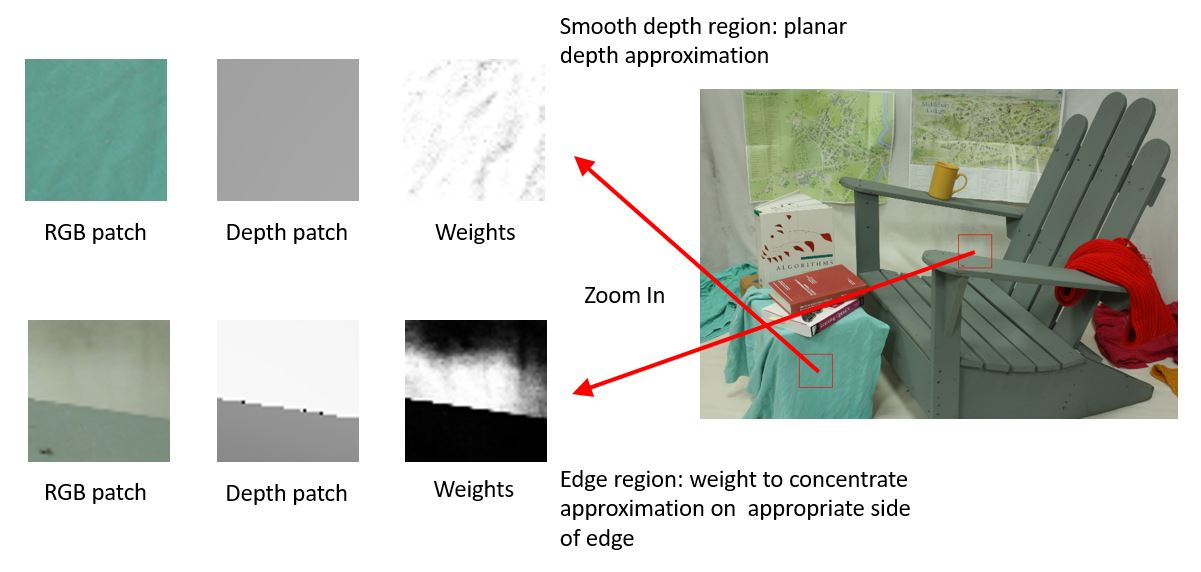
\includegraphics[width=0.95\linewidth]{depth_interp/misc/zoomin.JPG}
\label{fig2:zoomin}
\caption{The intuitive interpretation for the proposed algorithm. Two patch, respectively cropped from the handle area and the box ara, display different patterns in depth maps. The intuition of the proposed method aims to construct a linear interpolation based on only pixels with the same object which is supposed to be similar in both depth and color.}
\end{figure}
\begin{figure}[htb]
\centering
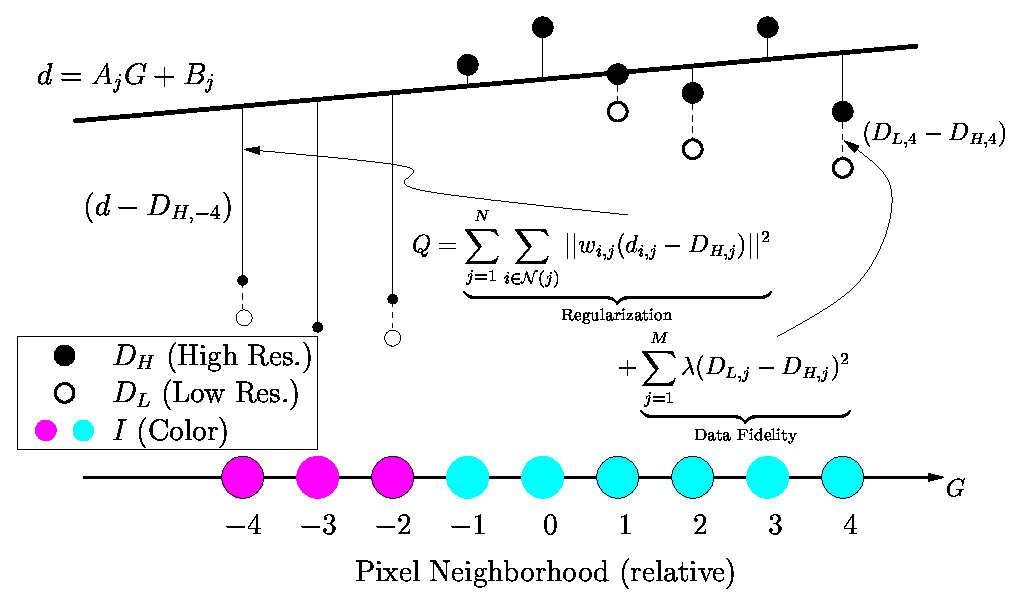
\includegraphics[width = 0.95\textwidth]{depth_interp/ProbFormulation.eps}
\vfill
\caption{The illustration of problem formulation in 1D. The magenta and cyan points show different color pixels in the patch of color image, and the circles around data points indicate the available low resolution depth values. The filled and un-filled circles mean the desired upsampled depth map and the input depth map, respectively, and the line is the fitting result on the example area. The weights are illustrated by the size of filled circles.}
\label{fig2:outline}
\end{figure}

To formally describe our algorithm we use the simplified 1D representation in Fig.~\ref{fig2:outline} that illustrates the contribution of one pixel to the objective function. The axis $G$ represents the relative pixel positions of points in local pixel neighborhood of the target pixel which is located at $G=0$. The low resolution depth map, denoted by $D_{L}$, is available at a subset of the pixel locations in the neighborhood as indicated in the figure and color values, denoted by $I$, form the high resolution RGB image. The goal is to estimate a high resolution depth map $D_H$. Our objective function is formulated as
\begin{equation}
Q = \sum_{j=1}^{N}{\sum_{i\in \mathcal{N}(j)}{||w_{i,j}(d_{i,j}-D_{H,i})||^2}}+\sum_{j=1}^{M}{{\lambda}(D_{L,j}-D_{H,j})^2},
\label{eq:2.1}
\end{equation}
where $j$ indexes the pixel locations in the upsampled image, $N$ is the number of pixels in the upsampled image, $M$ is the number of pixels in the low resolution depth map, $d_{i,j}$ is the value of linear fitting of pixel $i$ in the neighbor of pixel $j$, $D_{H,i}$ is the estimated depth at pixel $i$ in the neighbor of pixel $j$, and $D_{L,j}$ is the depth value at the pixel $j$ of the low resolution depth map, $w_{i,j}$ is the similarity metric of pixel $i$ and $j$, and $\lambda$ is the free parameter to control the relation of fidelity and smoothness. The local linear fit is defined as
\begin{equation}
d_{i,j} = A_{j}G_{i,j}+B_{j},
\label{eq:2.2}
\end{equation}
where $A_{j}$ and $B_{j}$ are the parameters for linear fitting at pixel $D_{H,j}$, $A_{j}$ is a 1-by-2 vector and $B_{j}$ is a scalar, and $G_{i,j}$ is a 2-by-1 vector denoting the relative coordinate of pixel $i$ in the neighbor window of pixel $j$. We define $G_{i,j}\overset{def}{=}\{(x,y)|-w_{s}<x<w_{s},-w_{s}<y<w_{s}\}$, where $w_{s}$ is the size of the window. The first term in~\eqref{eq:1} is the regularization term and the second term is the data fidelity. The formulation is readily extended to the hole filling problem by adding, to the fidelity penalty term, a product with the indicator function of non-missing points and pixel values.

The weights $w_{i,j}$ are defined as
\begin{equation}
w_{i,j} = \exp{-\frac{||I_{i}-I_{j}||^2}{2\sigma^2}},
\label{eq:2.4}
\end{equation}
where $I_{i}$ and $I_{j}$ are pixel values of the RGB image $I$ at corresponding position, and $\sigma$ controls the relative emphasis of pixel similarity in the allocation of weights. Alternative, formulations of the weights such as those used in non local mean or bilateral filter can also be used in the proposed framework. Unlike the typical bilateral filter, we do not use the distance decay term in~\eqref{eq:2.4} because the window we use is quite small comparing to the high resolution images. 

Our problem formulation and the algorithmic approach we use for the solution (described in the next section) are inspired by Levin's formulation of matting as an optimization problem~\cite{levin2008closed}, where the alpha channel is formulated as a weighted linear combination of neighboring color values. A key difference in our formulation is that the our weighted local linear fit is formulated in terms of the local relative {\em spatial} position for the neighborhood, whereas in~\cite{levin2008closed} the weighted linear fit is performed on the {\em color} values for the neighborhood pixels. 

\subsection{Optimization Solution}
\label{sec2.3.2}
%The optimization of this objective can be formulated as calculating the upsampling Laplacian matrix and solve the linear equation. 
Rewriting~\eqref{eq:2.1} in the matrix form, we obtain
\begin{equation}
Q = \sum_{j=1}^{N}{(W_{j}(D_{H,N_{j}}-GP_{j}^T))^2+{\lambda}F_{j}},
\label{eq:2.5}
\end{equation}
where $G = [G_j,1]$ and $P_{j} = [A_{j},B_{j}]^T$. $W_{j}$ is a diagonal matrix with $w_{i,j}$ being its diagonal entries. $D_{H,N_{j}}$ is the depth value in the patch\footnote{We pad the image to represent $G$ consistently at all positions.}. The matrix $P_{j}$ can be eliminated by replacing it in~\eqref{eq:2.5} by its optimal value 

\begin{equation}
\label{eq:2.6}
\begin{split}
P_{j} &=  {\argmin}_{P_{j}}{((W_{j}(D_{H,N_{j}}-GP_{j}^T))^2)}\\
&= (G^{T}W_{0,j}^{T}G)^{-1}G^{T}W_{0,j}^{T}D_{H,N_{j}},
\end{split}
\end{equation}
where $W_{0,j}$ is the diagonal matrix,
\begin{equation}
W_{0,j} = W_{j}^{T}W_{j},
\end{equation}
% \vspace*{-0.05in}
% \begin{equation*}
% W_{0,j} = W_{j}^{T}W_{j}.
% \vspace*{-0.05in}
% \end{equation*}

% As defined, $P_{j}$ is the fitting parameter based on the specific patch. By~\eqref{eq:6}, these terms have been expressed with known parameters.
Replacing $P_{j}$ in ~\eqref{eq:2.1} by~\eqref{eq:2.6}, we obtain,
\begin{equation}
Q = \sum_{j=1}^{N}{D_{H,N_{j}}^{T}(\overline{G_{j}}^{T}W_{0,j}\overline{G_{j}})D_{H,N_{j}}}+\sum_{j=1}^{M}{\lambda(D_{L,j}-D_{H,j})^2},
\label{eq:2.7}
\end{equation}
\begin{equation}
\overline{G_{j}}= E-G(G^{T}W_{0,j}^{T}G)^{-1}G^{T}W_{0,j},
\end{equation}
where $E$ denoting the identity matrix.
%can be expressed as
% \begin{equation*}
% \overline{G_{j}} = E-G(G^{T}W_{0,j}^{T}G)^{-1}G^{T}W_{0,j},
% \end{equation*}
% where $E$ is a identity matrix. At this point, all unknown parameters are eliminated and the optimization is just based on~\eqref{eq:5}.

%Because the objective function $Q$ is quadratic, 
The minimizer for the quadratic objective function $Q$ is readily obtained, specifically, as the solution to the linear equation,
\begin{equation}
LD+\lambda A(D-d) = 0,
\label{eq:2.8}
\end{equation}
where $L$ is the Laplacian matrix~\cite{merris1994laplacian},
\begin{equation}
L= \sum_{j=1}^{N}{\overline{G_{j}}^{T}W_{0,j}\overline{G_{j}}}
\label{eq:lpl}
\end{equation}
and $A$ is a diagonal matrix indicating the correspondence of pixels in low resolution map to the upsampled map. The derivation detail is listed in appendix~\ref{ap1}.
% is the 
% \begin{equation*}
% L = \sum_{j=1}^{N}{\overline{G_{j}}^{T}W_{0,j}\overline{G_{j}}},
% \end{equation*}
% and $A$ is a diagonal matrix indicating the correspondence of pixels in low resolution map to the upsampled map. $L$ is called the Laplacian matrix~\cite{merris1994laplacian}. With a proper window size, this linear equation is highly sparse and can be solved with conjugated gradient method.


%From the objective, we can see that depth map upsampling is similar to the matting problem~\cite{levin2008closed} with given strokes. The differences mainly lie in that in our algorithm, the depth value is linear to the relative position to the patch center and the color image working on the weight, while the matting algorithm directly formulates the alpha value on the linear combination of the color information.
\subsection{memory saving implementation}
\label{sec2.3.3}
In last section the optimization of the objective is formulated as an large sparse linear system, which can be efficiently solved with methods such as conjugate gradient solver. In practise, one important constraint for this method is that the Laplacian matrix and the successive processing, even though sparse, are very large and require a lot of memory. To reduce the memory requirement, we propose a computational efficiency improvement for the optimization, still exploiting the framework of conjugate gradient method~\cite{he2010fast,yu2014computational}.

Algorithm~\ref{algo:cg} describes the conjugate gradient algorithm for solving sparse linear systems. This algorithm is designed for solving symmetric and positive-definite linear systems, which is suitable for the optimization in our problem where the Laplacian matrix automatically satisfies the required condition. This method exploits the conjugate vectors with respect to $\textbf{A}$ and iteratively approximates the closest solution.

\begin{algorithm}
\SetKwData{Left}{left}
\SetKwData{This}{this}
\SetKwData{Up}{up}
\SetKwFunction{Union}{Union}
\SetKwFunction{FindCompress}{FindCompress}
\SetKwInOut{Input}{input}
\SetKwInOut{Output}{output}
\Input{Initial guess $\textbf{I}_0$, convergence threshold $\tau$}
\vspace{0.1in}
\Output{$\tilde{\textbf{I}}$ : estimate for $\textbf{I}$}
\vspace{0.1in}
\textbf{Procedure}\:
\vspace{0.1in}
\textbf{Initialize:} $\tilde{\textbf{I}}\leftarrow \textbf{I}_0$, $\textbf{r}_0\leftarrow \textbf{b}-\textbf{A}\tilde{\textbf{I}}$, $\textbf{p}_0\leftarrow \textbf{r}_0$, $j\leftarrow 0$\;
\vspace{0.1in}
\While{$\textbf{r}_j^T\textbf{r}_j > \tau |\textbf{I}|$}{\vspace{0.1in}$\alpha_j\leftarrow \frac{\textbf{r}_j^T\textbf{r}_j}{\textbf{p}_j^TA\textbf{p}_j}$\;\vspace{0.1in}
$\tilde{\textbf{I}}\leftarrow \tilde{\textbf{I}}+\alpha_j\textbf{p}_j$\;\vspace{0.1in}
$\textbf{r}_{j+1}\leftarrow \textbf{r}_j-\alpha_j \textbf{A}\textbf{p}_j$\;
\vspace{0.1in}
$\beta_j\leftarrow \frac{\textbf{r}_{j+1}^T\textbf{r}_{j+1}}{\textbf{r}_j^T\textbf{r}_j}$\;
\vspace{0.1in}
$\textbf{p}_{j+1}\leftarrow \textbf{r}_{j+1}+\beta_j \textbf{p}_j$\;\vspace{0.1in}}\vspace{0.1in}
\caption{Solve the sparse linear system $\textbf{AI} = \textbf{b}$ using conjugate-gradient algorithm.}
\label{algo:cg}
\end{algorithm}

One bottleneck for the proposed depth upsampling algorithm is that, for high resolution images, the Laplacian matrix is beyond typical computers' memory, for example a mega-pixel image will require constructing a matrix of tera-entries. This problem can be effective solved with some modifications on the naive conjugate gradient method, namely calculating $\textbf{A}\textbf{p}_j$ in algorithm~\ref{algo:cg} without explicit constructing $\textbf{A}$, in our case the Laplacian matrix.

From ~\eqref{eq:lpl} we can obtain the the entry $L_{i,j}$ at the $i$th row and the $j$ column of the Laplacian matrix, 
\begin{equation}
L_{i,j} = \sum_{k|i,j\in N_{k}}{(\delta_{ij}w_{ki}-w_{ki}w_{kj}(G_{i}-k_{0})C_{k}(G_{j}-k_{0}))},
\label{eq:2.cgs_partial1}
\end{equation}
where $N_{k}$ is the neighbour of pixel $k$, whose range is specified by the window size, $w_{ki}$ is the weigh of pixel $k$ to pixel $i$ and $j$, $\delta_{ij}$ is the Kronecker delta , $C_{k}$ is the inverse of $\overline{G_{j}}^{T}W_{0,j}\overline{G_{j}}$ of pixel $k$, $G_{i}$ is relative coordinate of pixel $i$ to $k$, and $k_0$ is the the global coordinate of the pixel $k$. Then we break the summation stepwise, first computing, 
\begin{equation}
a_{k} = C_{k}(\sum_{j\in N_{k}}{w_{kj}}G_{j}P_{j}-k\overline{p_{k}}),
\label{eq:2.cgs_partial2}
\end{equation}
where $P_j$ is the $i$th entry of vector $P$, and $\overline{p_{k}}$ is the average of $P_j$ in $N_{k}$. then,
\begin{equation}
b_{k} = k_{0}a_{k},
\label{eq:2.cgs_partial3}
\end{equation}
at the last step, combine $a_k$ and $b_k$ to obtain $(Lp)_{i}$, the entry at the $i$th column of vector $Lp$,
\begin{equation}
(Lp)_{i} = \sum{\delta_{ij}w_{ki}P_{i}}-G_{i}\sum_{k\in N_{i}}{a_{k}w_{ki}}+\sum_{k\in N_{i}}{b_{k}w_{ki}},
\label{eq:2.cgs_final}
\end{equation}
further, the inverse $C_k$ can be expressed as,
\begin{landscape}
\begin{equation}
C = \left \{
  \begin{tabular}{ccc}
  $\textbf{y}^T\textbf{wy1}^T\textbf{w1}-\textbf{y}^T\textbf{w11}^T\textbf{wy}$ & $\textbf{y}^T\textbf{w11}^T\textbf{wx}-\textbf{y}^T\textbf{wx1}^T\textbf{w1}$ & $\textbf{y}^T\textbf{wx1}^T\textbf{wy}-\textbf{y}^T\textbf{wy1}^T\textbf{wx}$ \\
  $\textbf{x}^T\textbf{w11}^T\textbf{wy}-\textbf{x}^T\textbf{wy1}^T\textbf{w1}$ & $\textbf{x}^T\textbf{wx1}^T\textbf{w1}-\textbf{x}^T\textbf{w11}^T\textbf{wx}$ & $\textbf{x}^T\textbf{wy1}^T\textbf{wx}-\textbf{x}^T\textbf{wx1}^T\textbf{wy}$ \\
  $\textbf{x}^T\textbf{wyy}^T\textbf{w1}-\textbf{x}^T\textbf{w1y}^T\textbf{wy}$ & $\textbf{x}^T\textbf{w1y}^T\textbf{wx}-\textbf{x}^T\textbf{wxy}^T\textbf{w1}$ & $\textbf{x}^T\textbf{wxy}^T\textbf{wy}-\textbf{x}^T\textbf{wyy}^T\textbf{wx}$
  \end{tabular}
\right \},\\
\label{eq:2.inverse}
\end{equation}
or more compactly as the minor of the matrix:\\
\begin{equation}
C = \left \{
  \begin{tabular}{ccc}
  $M_{1,1}$ & $M_{1,2}$ & $M_{1,3}$ \\
  $M_{2,1}$ & $M_{2,2}$ & $M_{2,3}$ \\
  $M_{3,1}$ & $M_{3,2}$ & $M_{3,3}$
  \end{tabular}
\right \},
\end{equation}
here the normalization term omitted.
\end{landscape}
Substitute the update step of $p_{j+1}$ in algorithm~\ref{algo:cg} with~\eqref{eq:2.cgs_final} we can get the version for optimization the proposed depth upsampling algorithm. The derivation detail is listed in appendix~\ref{ap2}.

In colorization problem the summation in~\eqref{eq:2.cgs_partial2},~\eqref{eq:2.cgs_partial3}, and ~\eqref{eq:2.cgs_final} can be efficiently calculated by integral image techniques and dynamic programming. This step is possible as that the formulation in colorization utilizes a fixed summation table; but in our case, the $G_{j}w_{kj}$ is a summed table of localized filters $w_{k}$, which means that the values re-used in summed table is no longer applicable here. This restriction limits the acceleration of computing but still allows the memory saving. By this implementation the required memory for a two mega-pixel image is reduced from 60GB to 2GB memory. With parallel computation, this method can have a good balance in memory usage and time consumption.


\section{experimental results}
\label{sec:2.result}
We test our algorithm on the Middlebury (stereo) dataset~\cite{scharstein2003high,scharstein2007learning,hirschmuller2007evaluation,scharstein2014high}, which provides high resolution RGB images of multiple views and corresponding disparity maps, which are used as the ground truth in our experiment. We use a window size of $7\times 7$ ($\equiv N=49$), and $\lambda=10^5$. The RGB-D images are zero-padded for consistent use of~\eqref{eq:5}, and the padded area is cropped out in the final results. The parameter $\sigma^2$ in~\eqref{eq:4} for computation of the weights $w_{i,j}$ is set to one third of the local variance in each window. In each patch, the weight of the center pixel is set to $10^{-5}$. We use the built-in Matlab conjugate gradient solver (\emph{cgs}) for solving~\eqref{eq:8} (a tolerance of $10^{-10}$ and maximum number of iteration $10^4$ were used).
\subsection{Qualitative and Quantitative Results}
The proposed algorithm is both suitable for hole filling for single disparity map and depth map upsampling, as indicated earlier. In this part, we first visually examine the performance of filling holes in depth map, as shown in Fig.~\ref{fig:quali_rst}. From the images in the last column, we can find that the holes, which correspond to the occluded area in the disparity map, are well filled. Unlike traditional interpolation methods, our algorithm is able to fix the holes in the depth images, so as to keep the consistency of depth map edges with those in the RGB images and avoid smoothing in such areas. For example, see the third row of Fig.~\ref{fig:quali_rst}. The missing points along the wall are well fitted to the two sides, and not blurred as a large patch.
% Behind we show results of the interpolation.
\begin{figure}[htb]
% \begin{minipage}[b]{0.3\linewidth}
%   \centering
%   \centerline{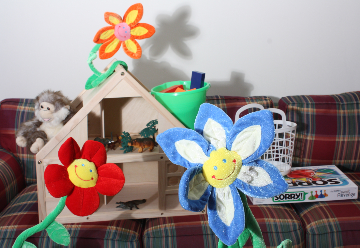
\includegraphics[width=2.7cm]{quali_rst/img_Flowers-perfect.png}}
% %  \vspace{1.5cm}
% %   \centerline{(a)}\medskip
% \end{minipage}
% %
% \hfill
% \begin{minipage}[b]{0.3\linewidth}
%   \centering
%   \centerline{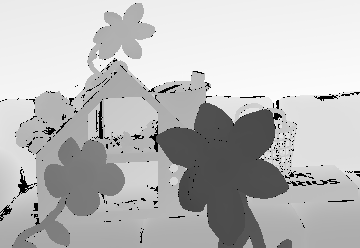
\includegraphics[width=2.7cm]{quali_rst/n_hf_Flowers-perfect.png}}
% %  \vspace{1.5cm}
% %   \centerline{(b)}\medskip
% \end{minipage}
% \hfill
% \begin{minipage}[b]{0.3\linewidth}
%   \centering
%   \centerline{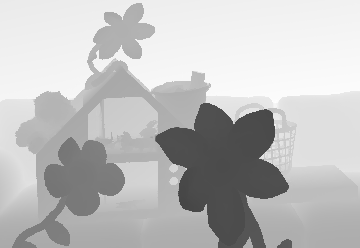
\includegraphics[width=2.7cm]{quali_rst/hf_Flowers-perfect.png}}
% %  \vspace{1.5cm}
% %   \centerline{(c)}\medskip
% \end{minipage}
% \vfill
\begin{minipage}[b]{0.3\linewidth}
  \centering
  \centerline{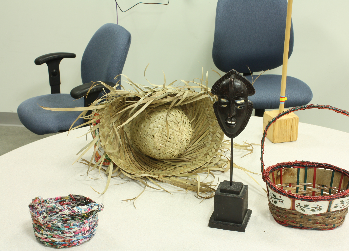
\includegraphics[width=4.2cm]{depth_interp/quali_rst/img_Mask-perfect.png}}
%  \vspace{1.5cm}
%   \centerline{(a)}\medskip
\end{minipage}
%
\hfill
\begin{minipage}[b]{0.3\linewidth}
  \centering
  \centerline{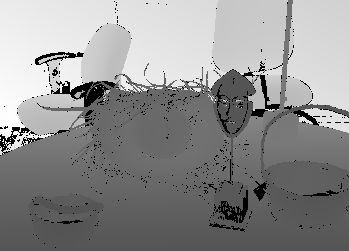
\includegraphics[width=4.2cm]{depth_interp/quali_rst/n_hf_Mask-perfect.png}}
%  \vspace{1.5cm}
%   \centerline{(b)}\medskip
\end{minipage}
\hfill
\begin{minipage}[b]{0.3\linewidth}
  \centering
  \centerline{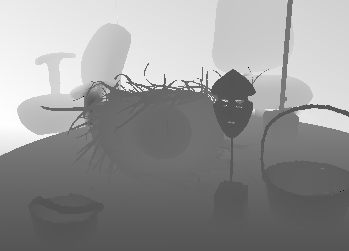
\includegraphics[width=4.2cm]{depth_interp/quali_rst/hf_Mask-perfect.png}}
%  \vspace{1.5cm}
%   \centerline{(c)}\medskip
\end{minipage}
\vfill
% \begin{minipage}[b]{0.3\linewidth}
%   \centering
%   \centerline{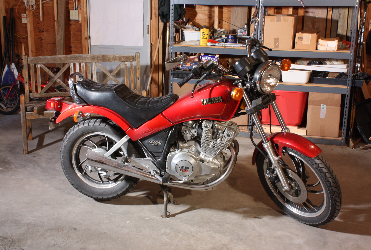
\includegraphics[width=2.7cm]{quali_rst/img_Motorcycle-perfect.png}}
% %  \vspace{1.5cm}
% %   \centerline{(a)}\medskip
% \end{minipage}
% %
% \hfill
% \begin{minipage}[b]{0.3\linewidth}
%   \centering
%   \centerline{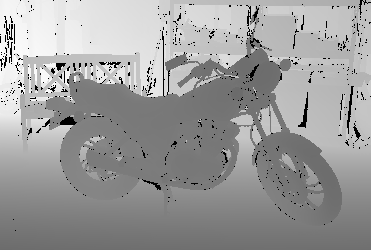
\includegraphics[width=2.7cm]{quali_rst/n_hf_Motorcycle-perfect.png}}
% %  \vspace{1.5cm}
% %   \centerline{(b)}\medskip
% \end{minipage}
% \hfill
% \begin{minipage}[b]{0.3\linewidth}
%   \centering
%   \centerline{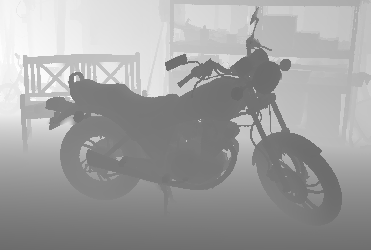
\includegraphics[width=2.7cm]{quali_rst/hf_Motorcycle-perfect.png}}
% %  \vspace{1.5cm}
% %   \centerline{(c)}\medskip
% \end{minipage}
% \vfill
\begin{minipage}[b]{0.3\linewidth}
  \centering
  \centerline{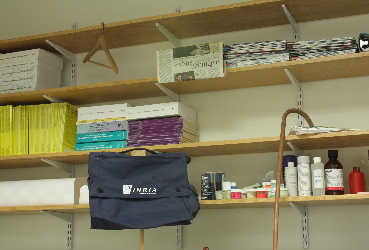
\includegraphics[width=4.2cm]{depth_interp/quali_rst/img_Shelves-perfect.png}}
%  \vspace{1.5cm}
%   \centerline{(a)}\medskip
\end{minipage}
%
\hfill
\begin{minipage}[b]{0.3\linewidth}
  \centering
  \centerline{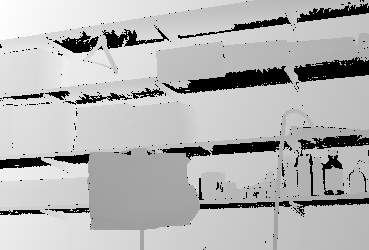
\includegraphics[width=4.2cm]{depth_interp/quali_rst/n_hf_Shelves-perfect.png}}
%  \vspace{1.5cm}
%   \centerline{(b)}\medskip
\end{minipage}
\hfill
\begin{minipage}[b]{0.3\linewidth}
  \centering
  \centerline{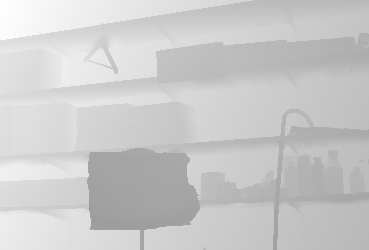
\includegraphics[width=4.2cm]{depth_interp/quali_rst/hf_Shelves-perfect.png}}
%  \vspace{1.5cm}
%   \centerline{(c)}\medskip
\end{minipage}
\vfill
\begin{minipage}[b]{0.3\linewidth}
  \centering
  \centerline{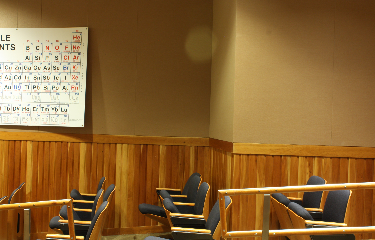
\includegraphics[width=4.2cm]{depth_interp/quali_rst/img_Classroom1-perfect.png}}
%  \vspace{1.5cm}
%   \centerline{(a)}\medskip
\end{minipage}
%
\hfill
\begin{minipage}[b]{0.3\linewidth}
  \centering
  \centerline{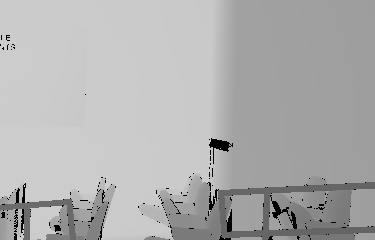
\includegraphics[width=4.2cm]{depth_interp/quali_rst/n_hf_Classroom1-perfect.png}}
%  \vspace{1.5cm}
%   \centerline{(b)}\medskip
\end{minipage}
\hfill
\begin{minipage}[b]{0.3\linewidth}
  \centering
  \centerline{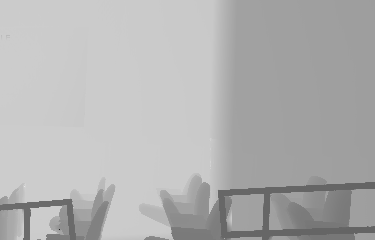
\includegraphics[width=4.2cm]{depth_interp/quali_rst/hf_Classroom1-perfect.png}}
%  \vspace{1.5cm}
%   \centerline{(c)}\medskip
\end{minipage}
\vfill
\begin{minipage}[b]{0.3\linewidth}
  \centering
  \centerline{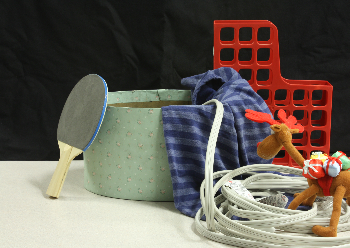
\includegraphics[width=4.2cm]{depth_interp/quali_rst/img_Cable-perfect.png}}
%  \vspace{1.5cm}
%   \centerline{(a)}\medskip
\end{minipage}
%
\hfill
\begin{minipage}[b]{0.3\linewidth}
  \centering
  \centerline{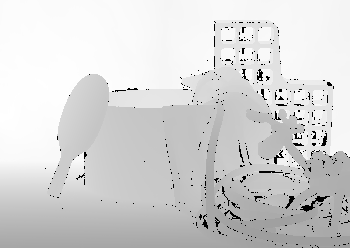
\includegraphics[width=4.2cm]{depth_interp/quali_rst/n_hf_Cable-perfect.png}}
%  \vspace{1.5cm}
%   \centerline{(b)}\medskip
\end{minipage}
\hfill
\begin{minipage}[b]{0.3\linewidth}
  \centering
  \centerline{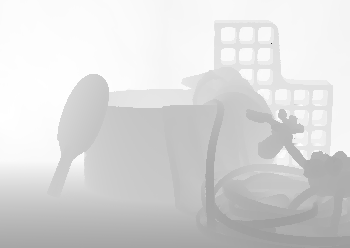
\includegraphics[width=4.2cm]{depth_interp/quali_rst/hf_Cable-perfect.png}}
%  \vspace{1.5cm}
%   \centerline{(c)}\medskip
\end{minipage}
\vspace*{-0.10in}
\caption{Qualitative results of the hole filling ability of our algorithm, tested on Middlebury stereo dataset 2014~\cite{scharstein2014high}. The first column shows the input high resolution color images and the second column shows the corresponding depth maps. The results are shown in the last column. The images are processed at a low resolution of approximate 60k to 80k pixels.}
\label{fig:quali_rst}
\end{figure}
\begin{figure*}[t]
\begin{minipage}[b]{1.0\linewidth}
  \centering
  \centerline{\includegraphics[width=6cm]{depth_interp/quan_hf/Art.png}}
%  \vspace{1.5cm}
%   \centerline{(a)}\medskip
\end{minipage}
%
\vfill
\begin{minipage}[b]{0.48\linewidth}
  \centering
  \centerline{\includegraphics[width=5.5cm]{depth_interp/quan_nhf/gt.png}}
%  \vspace{1.5cm}
%   \centerline{(a)}\medskip
\end{minipage}
\hfill
\begin{minipage}[b]{0.48\linewidth}
  \centering
  \centerline{\includegraphics[width=5.5cm]{depth_interp/quan_nhf/bl.png}}
%  \vspace{1.5cm}
%   \centerline{(a)}\medskip
\end{minipage}
%
\vfill
\begin{minipage}[b]{0.48\linewidth}
  \centering
  \centerline{\includegraphics[width=5.5cm]{depth_interp/quan_nhf/bc.png}}
%  \vspace{1.5cm}
%   \centerline{(b)}\medskip
\end{minipage}
\hfill
\begin{minipage}[b]{0.48\linewidth}
  \centering
  \centerline{\includegraphics[width=5.5cm]{depth_interp/quan_nhf/yang.png}}
%  \vspace{1.5cm}
%   \centerline{(a)}\medskip
\end{minipage}
%
\vfill
\begin{minipage}[b]{0.48\linewidth}
  \centering
  \centerline{\includegraphics[width=5.5cm]{depth_interp/quan_nhf/tgv.png}}
%  \vspace{1.5cm}
%   \centerline{(a)}\medskip
\end{minipage}
%
\hfill
\begin{minipage}[b]{0.48\linewidth}
  \centering
  \centerline{\includegraphics[width=5.5cm]{depth_interp/quan_nhf/our.png}}
%  \vspace{1.5cm}
%   \centerline{(b)}\medskip
\end{minipage}
\vfill
\label{fig2:art}
\caption{Visual comparison of different algorithm tested on Middlebury dataset~\cite{scharstein2003high} at $4\times$ upsampling rate. Column from left to right: RGB images, ground truth, and the results of: bilinear, bicubic, IBL~\cite{yang2014color}, TGV~\cite{ferstl2013image} and proposed; row from top to bottom: Art, Books, and Moebius.}
\end{figure*}
\begin{figure*}[t]
\begin{minipage}[b]{1\linewidth}
  \centering
  \centerline{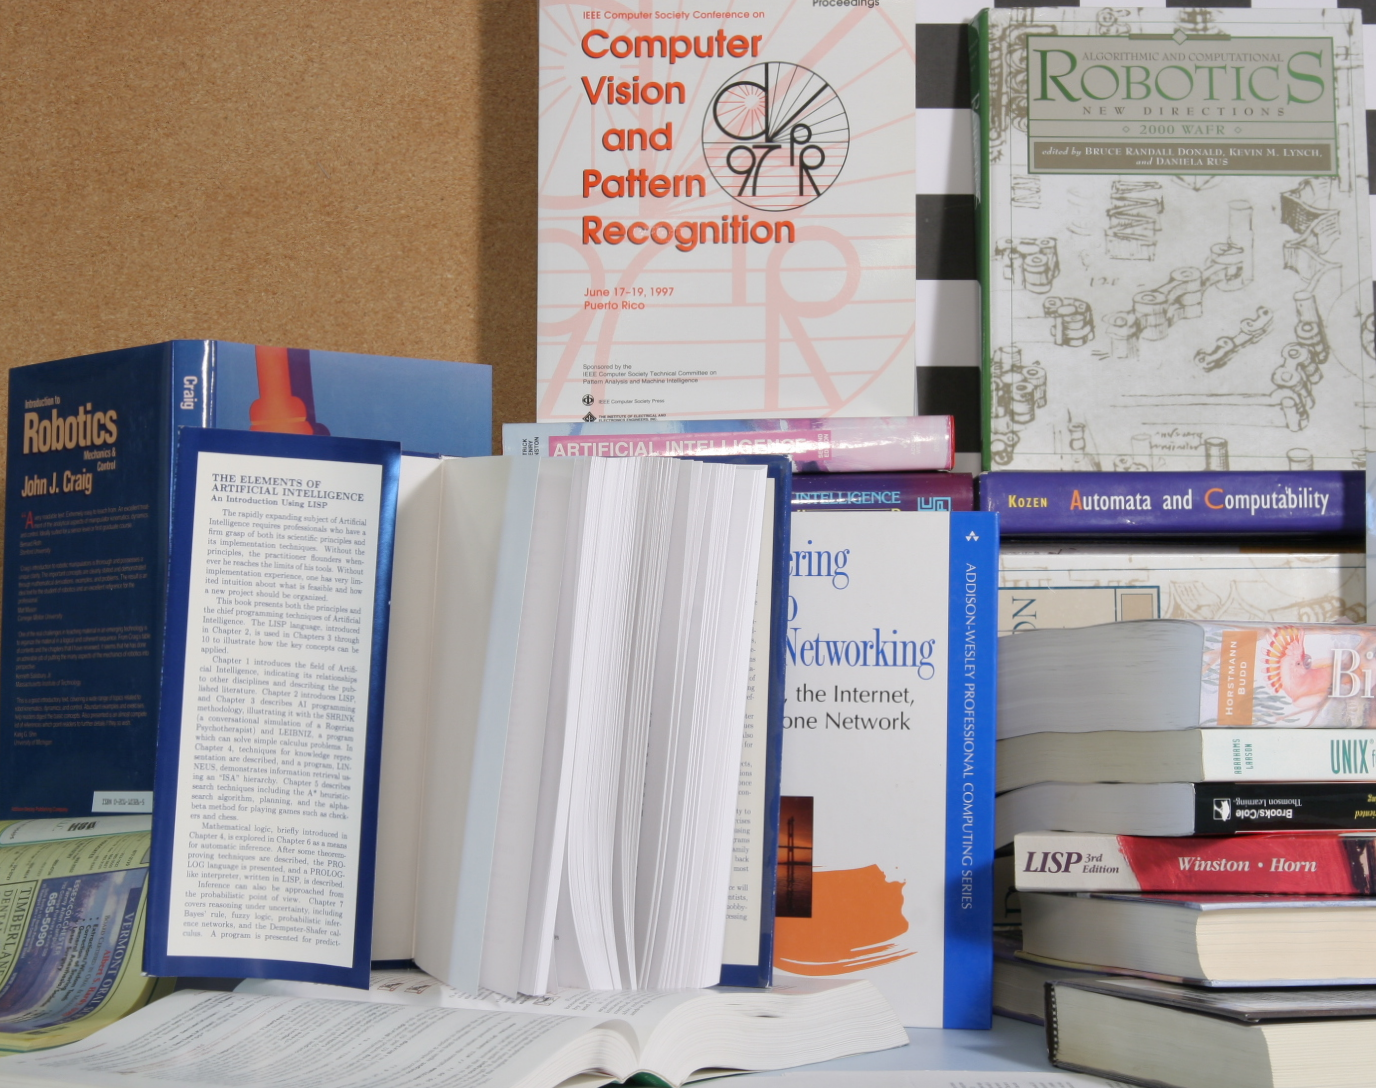
\includegraphics[width=6cm]{depth_interp/quan_nhf_books/Books.png}}
%  \vspace{1.5cm}
%   \centerline{(c)}\medskip
\end{minipage}
\hfill
\begin{minipage}[b]{0.48\linewidth}
  \centering
  \centerline{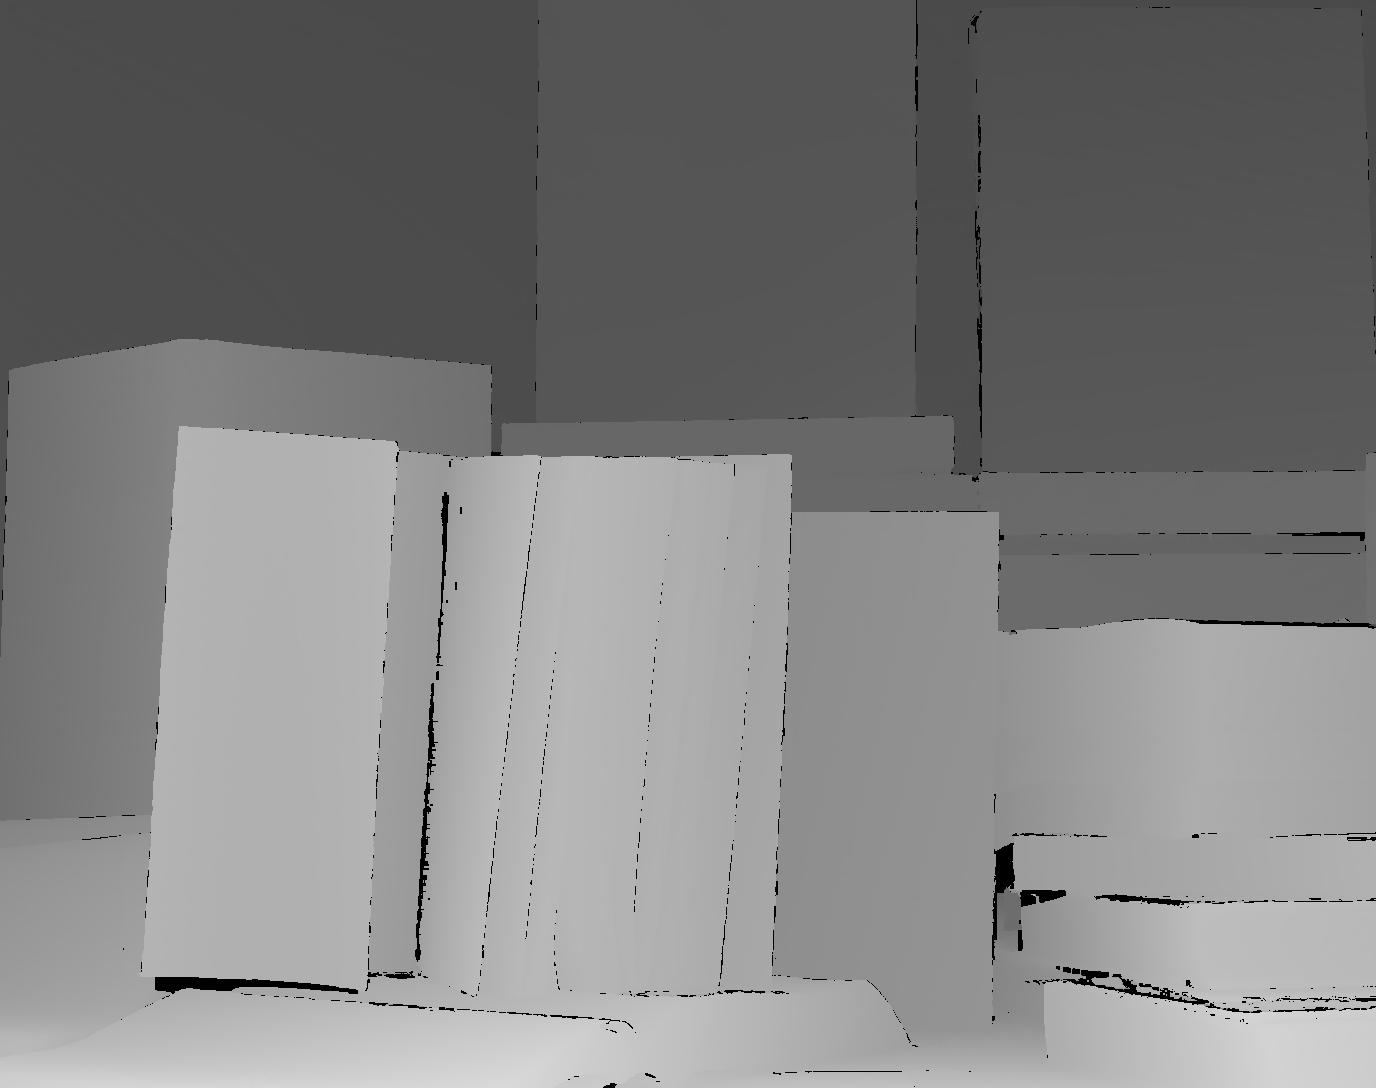
\includegraphics[width=5.5cm]{depth_interp/quan_nhf_books/gt.png}}
%  \vspace{1.5cm}
%   \centerline{(c)}\medskip
\end{minipage}
\hfill
\begin{minipage}[b]{0.48\linewidth}
  \centering
  \centerline{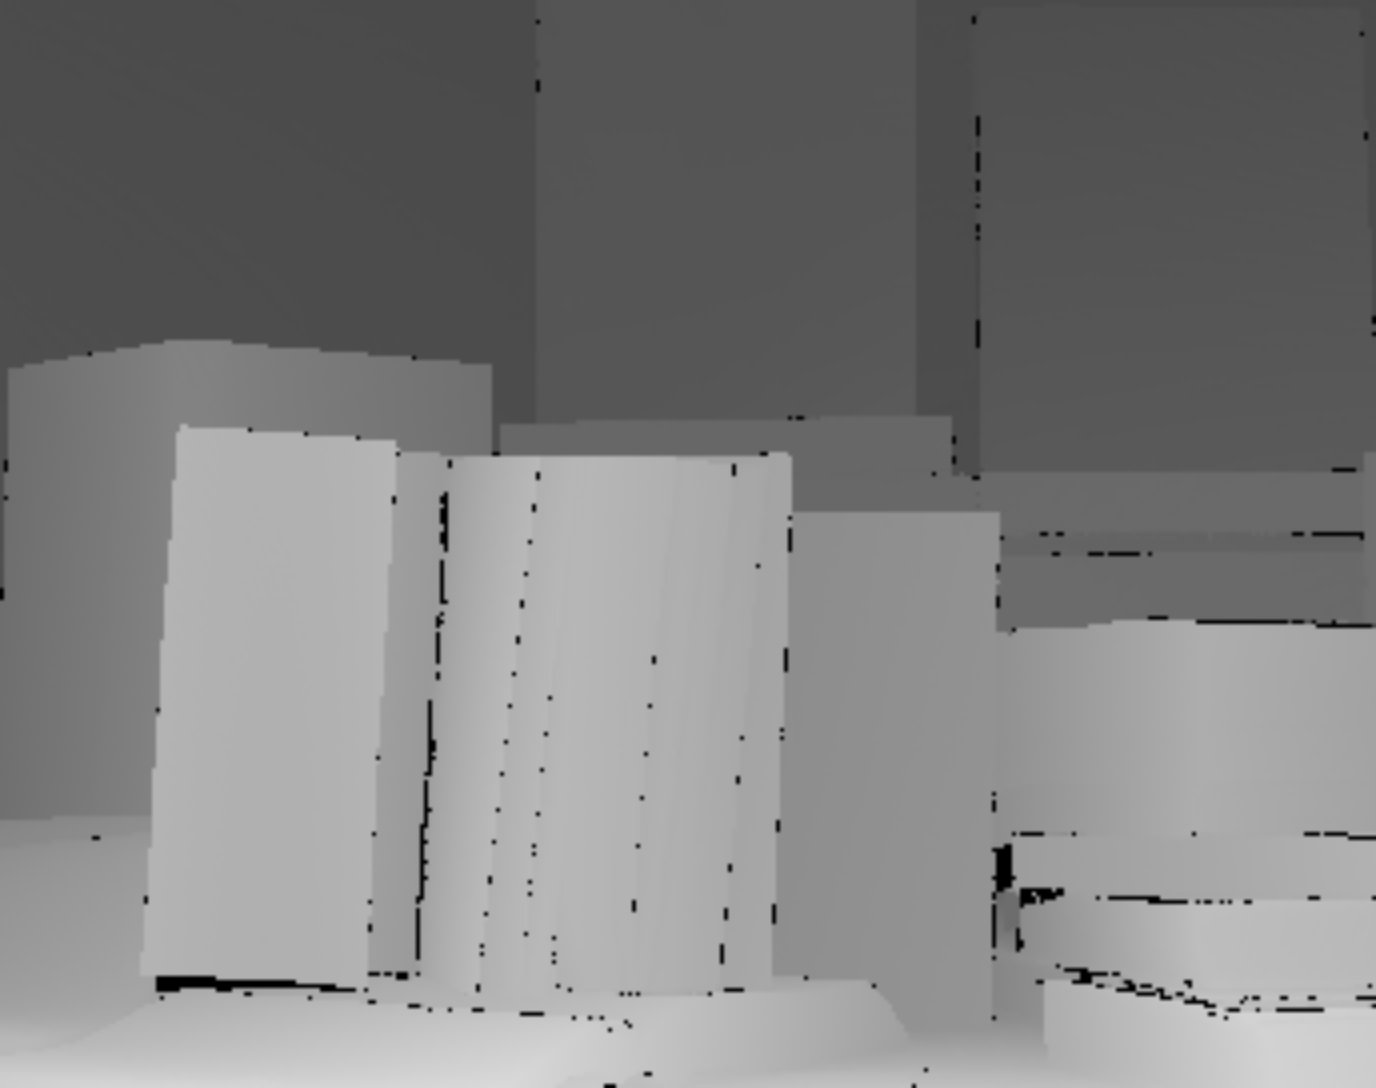
\includegraphics[width=5.5cm]{depth_interp/quan_nhf_books/bl.png}}
%  \vspace{1.5cm}
%   \centerline{(a)}\medskip
\end{minipage}
%
\hfill
\begin{minipage}[b]{0.48\linewidth}
  \centering
  \centerline{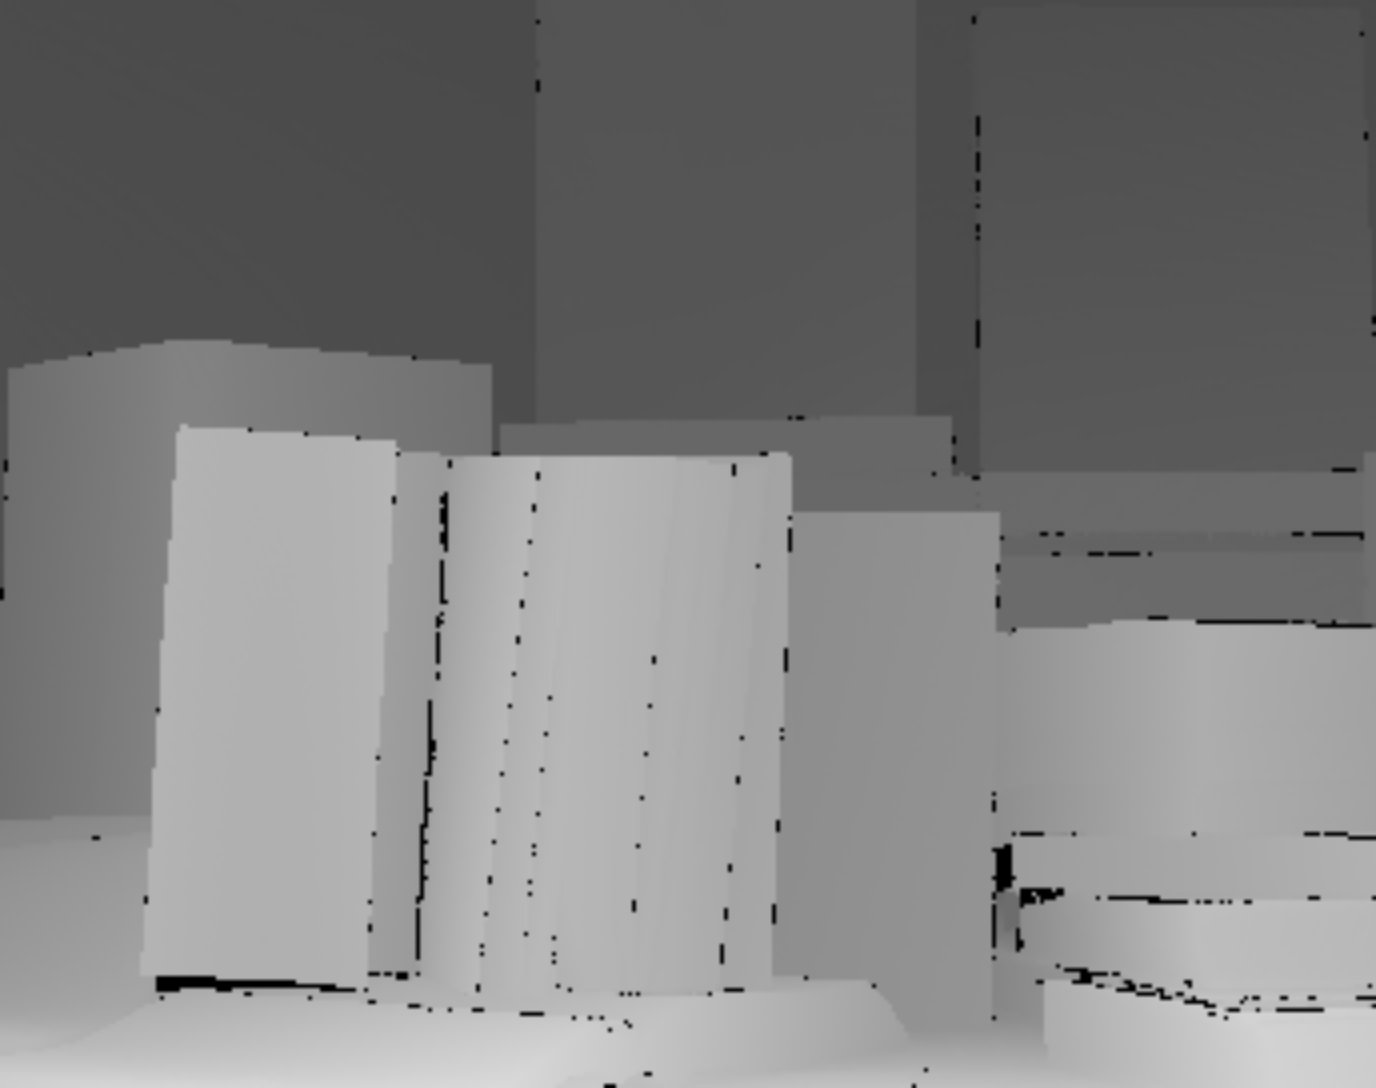
\includegraphics[width=5.5cm]{depth_interp/quan_nhf_books/bc.png}}
%  \vspace{1.5cm}
%   \centerline{(b)}\medskip
\end{minipage}
\hfill
\begin{minipage}[b]{0.48\linewidth}
  \centering
  \centerline{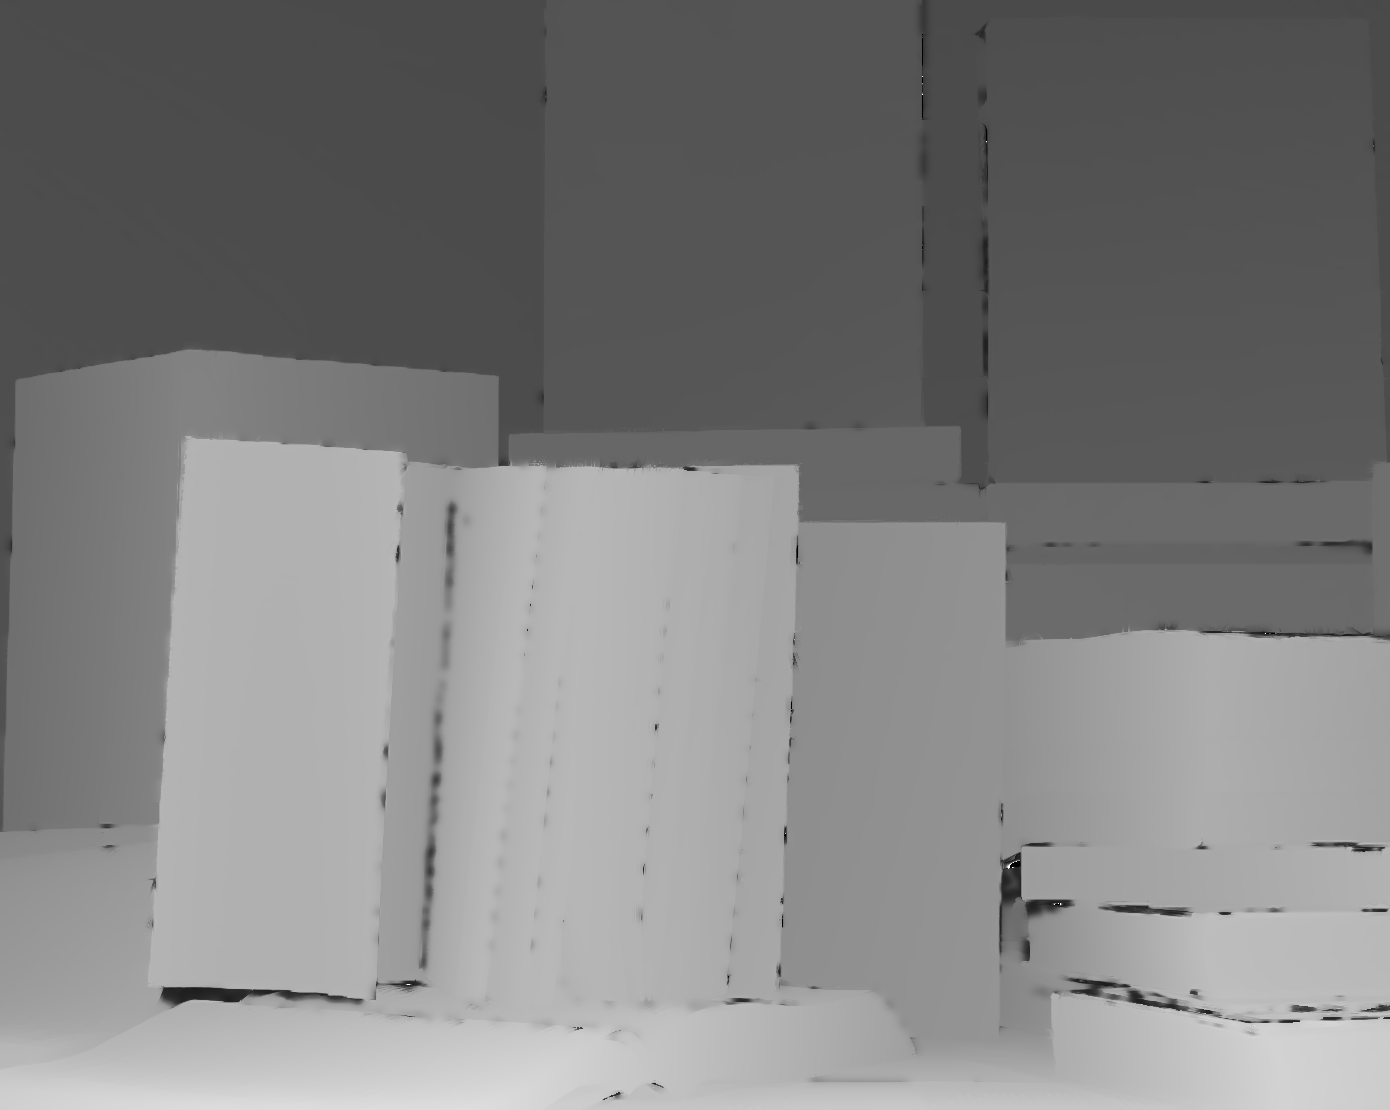
\includegraphics[width=5.5cm]{depth_interp/quan_nhf_books/yang.png}}
%  \vspace{1.5cm}
%   \centerline{(a)}\medskip
\end{minipage}
%
\hfill
\begin{minipage}[b]{0.48\linewidth}
  \centering
  \centerline{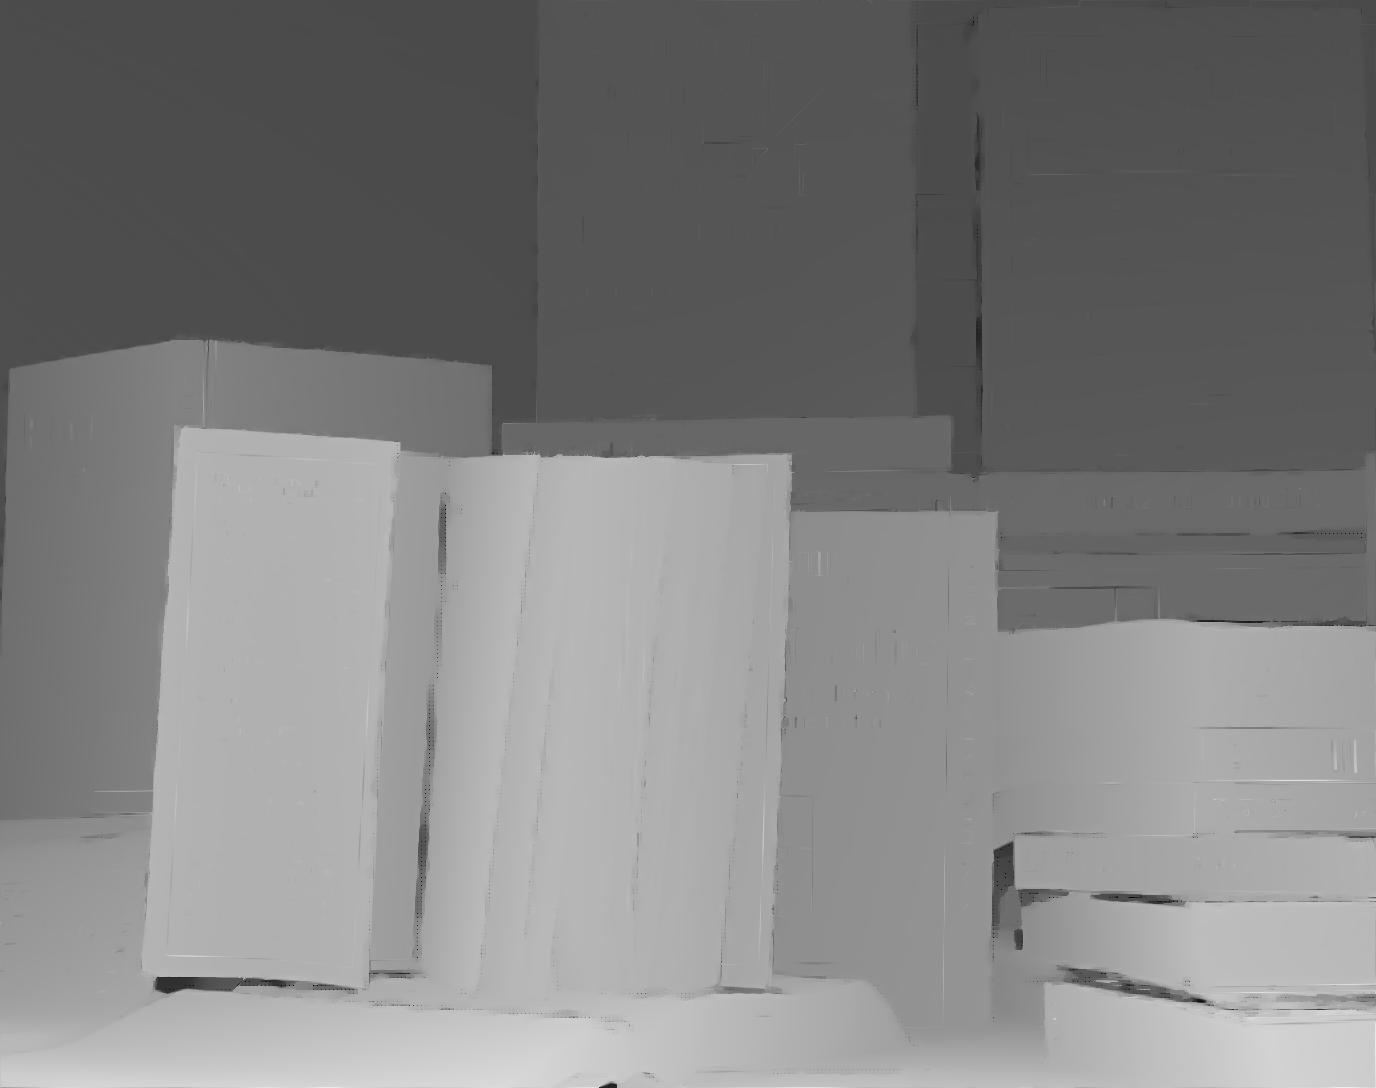
\includegraphics[width=5.5cm]{depth_interp/quan_nhf_books/tgv.png}}
%  \vspace{1.5cm}
%   \centerline{(a)}\medskip
\end{minipage}
%
\hfill
\begin{minipage}[b]{0.48\linewidth}
  \centering
  \centerline{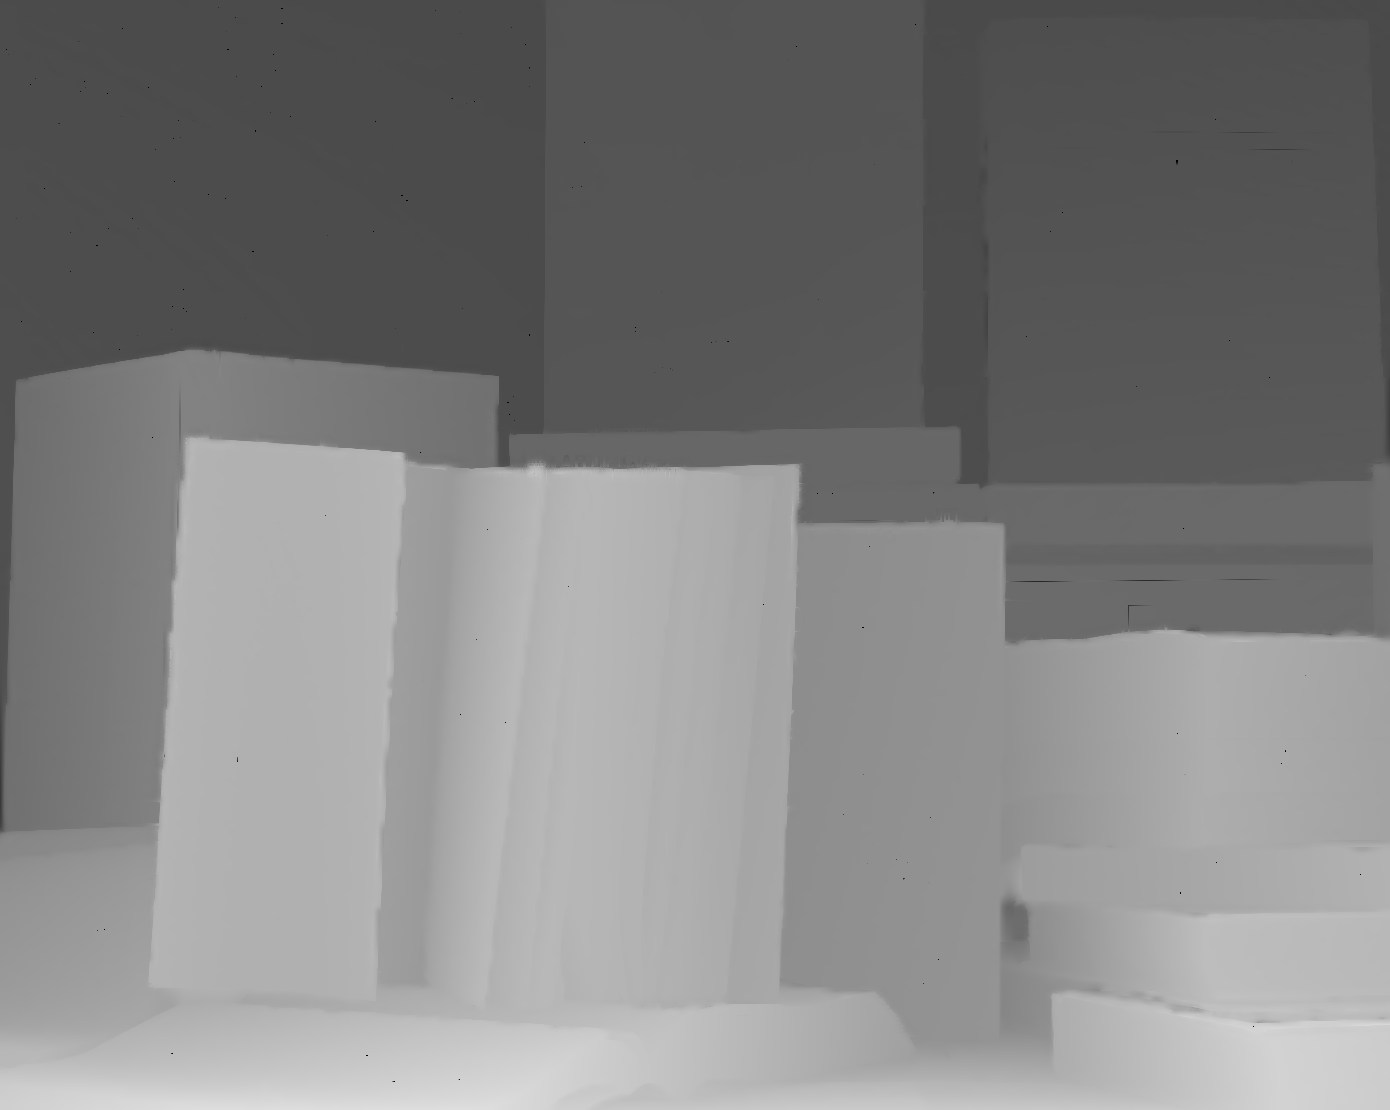
\includegraphics[width=5.5cm]{depth_interp/quan_nhf_books/our.png}}
%  \vspace{1.5cm}
%   \centerline{(b)}\medskip
\end{minipage}
\vfill
\label{fig2:books}
\caption{Visual comparison of different algorithm tested on Middlebury dataset~\cite{scharstein2003high} at $4\times$ upsampling rate. Column from left to right: RGB images, ground truth, and the results of: bilinear, bicubic, IBL~\cite{yang2014color}, TGV~\cite{ferstl2013image} and proposed; row from top to bottom: Art, Books, and Moebius.}
\end{figure*}
\begin{figure*}[t]
\begin{minipage}[b]{1\linewidth}
  \centering
  \centerline{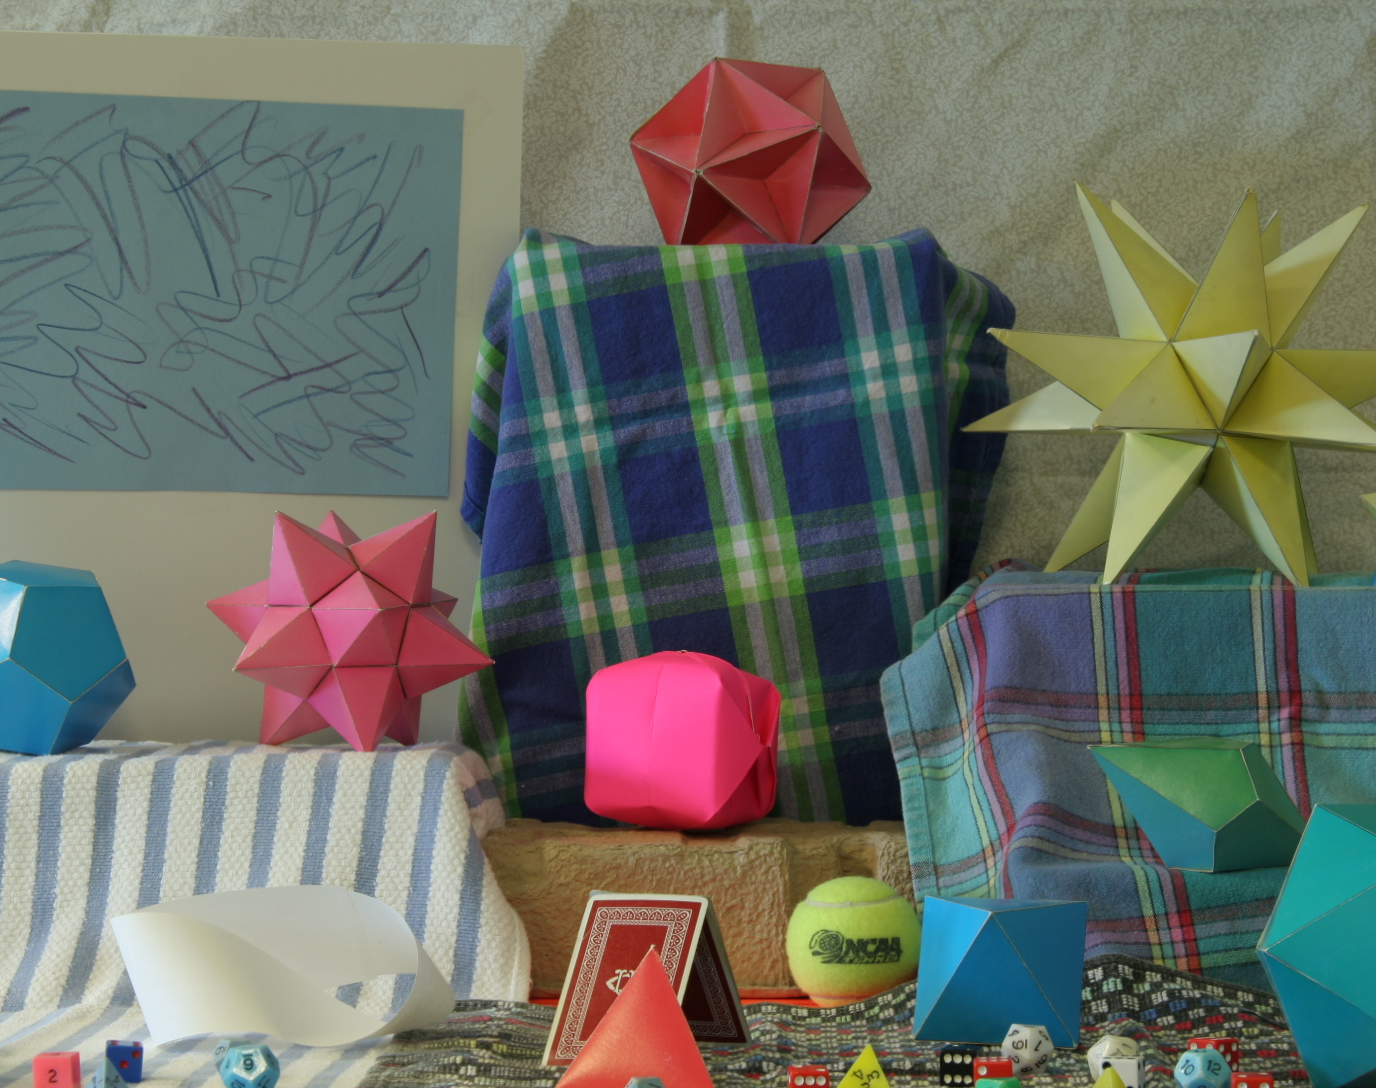
\includegraphics[width=6cm]{depth_interp/quan_nhf_moebius/Moebius.png}}
%  \vspace{1.5cm}
%   \centerline{(c)}\medskip
\end{minipage}
\hfill
\begin{minipage}[b]{0.48\linewidth}
  \centering
  \centerline{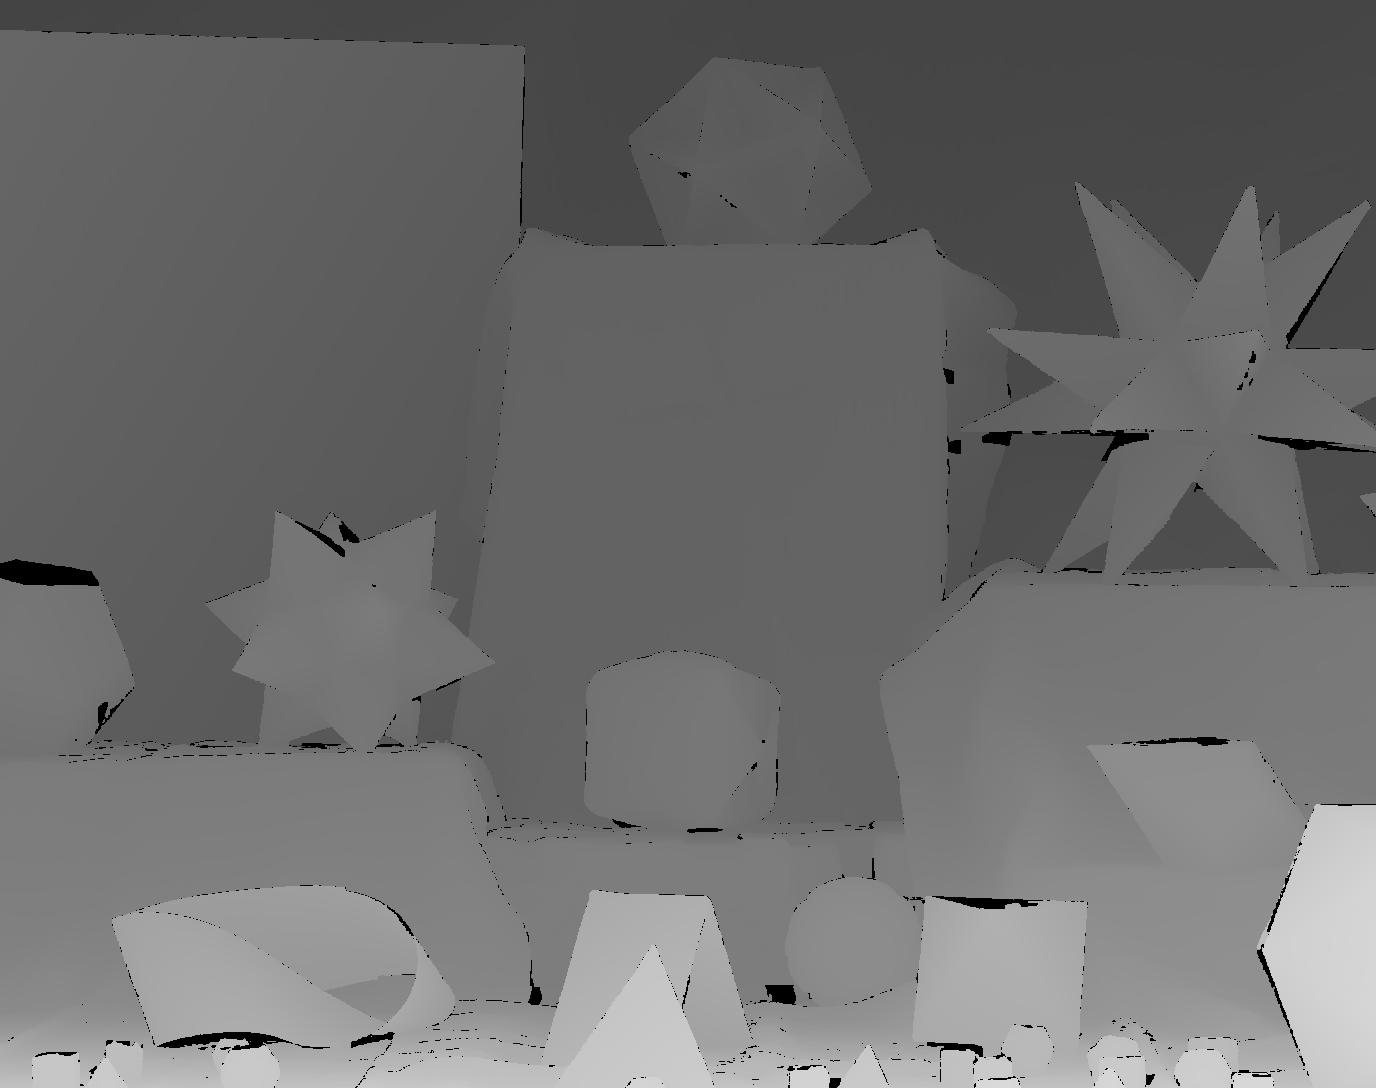
\includegraphics[width=5.5cm]{depth_interp/quan_nhf_moebius/gt.png}}
%  \vspace{1.5cm}
%   \centerline{(c)}\medskip
\end{minipage}
\hfill
\begin{minipage}[b]{0.48\linewidth}
  \centering
  \centerline{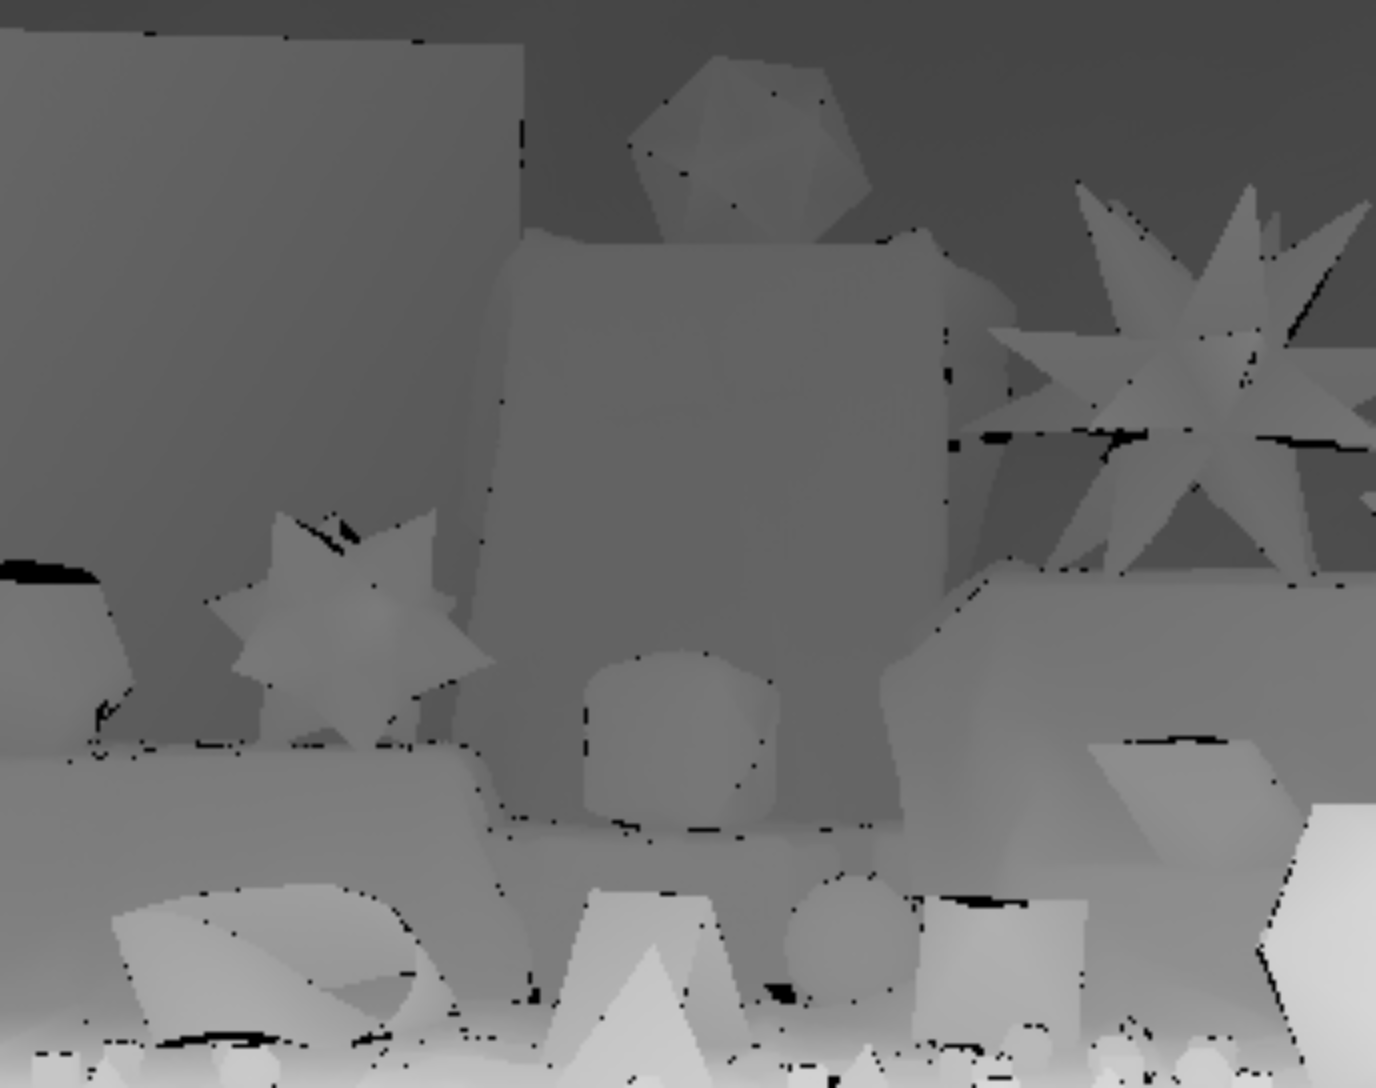
\includegraphics[width=5.5cm]{depth_interp/quan_nhf_moebius/bl.png}}
%  \vspace{1.5cm}
%   \centerline{(a)}\medskip
\end{minipage}
%
\hfill
\begin{minipage}[b]{0.48\linewidth}
  \centering
  \centerline{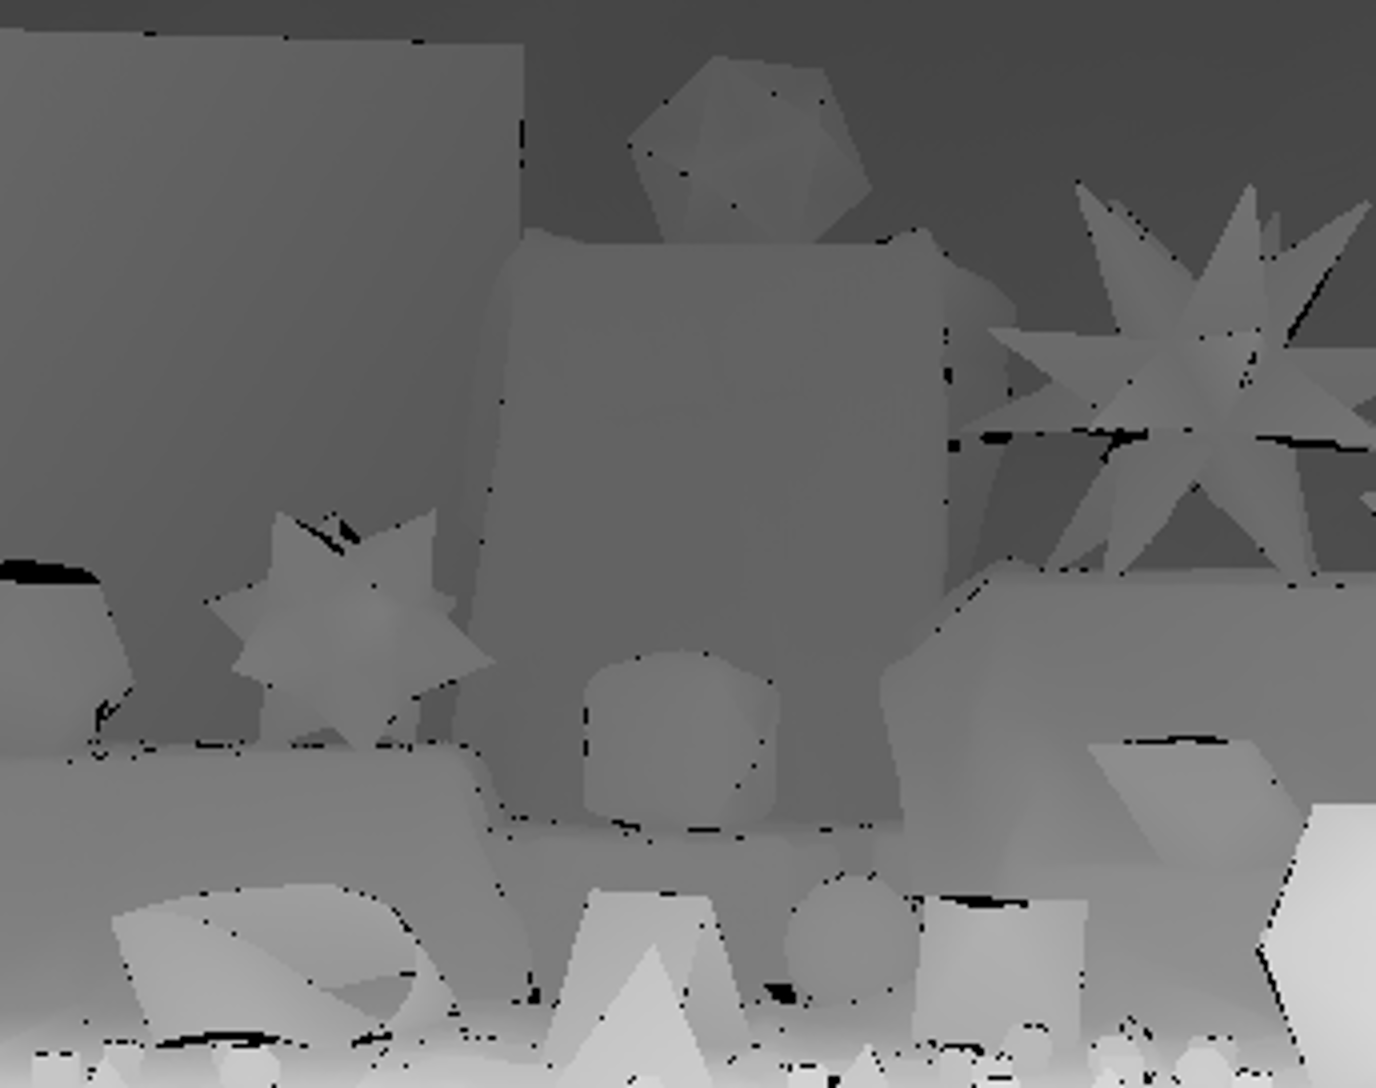
\includegraphics[width=5.5cm]{depth_interp/quan_nhf_moebius/bc.png}}
%  \vspace{1.5cm}
%   \centerline{(b)}\medskip
\end{minipage}
\hfill
\begin{minipage}[b]{0.48\linewidth}
  \centering
  \centerline{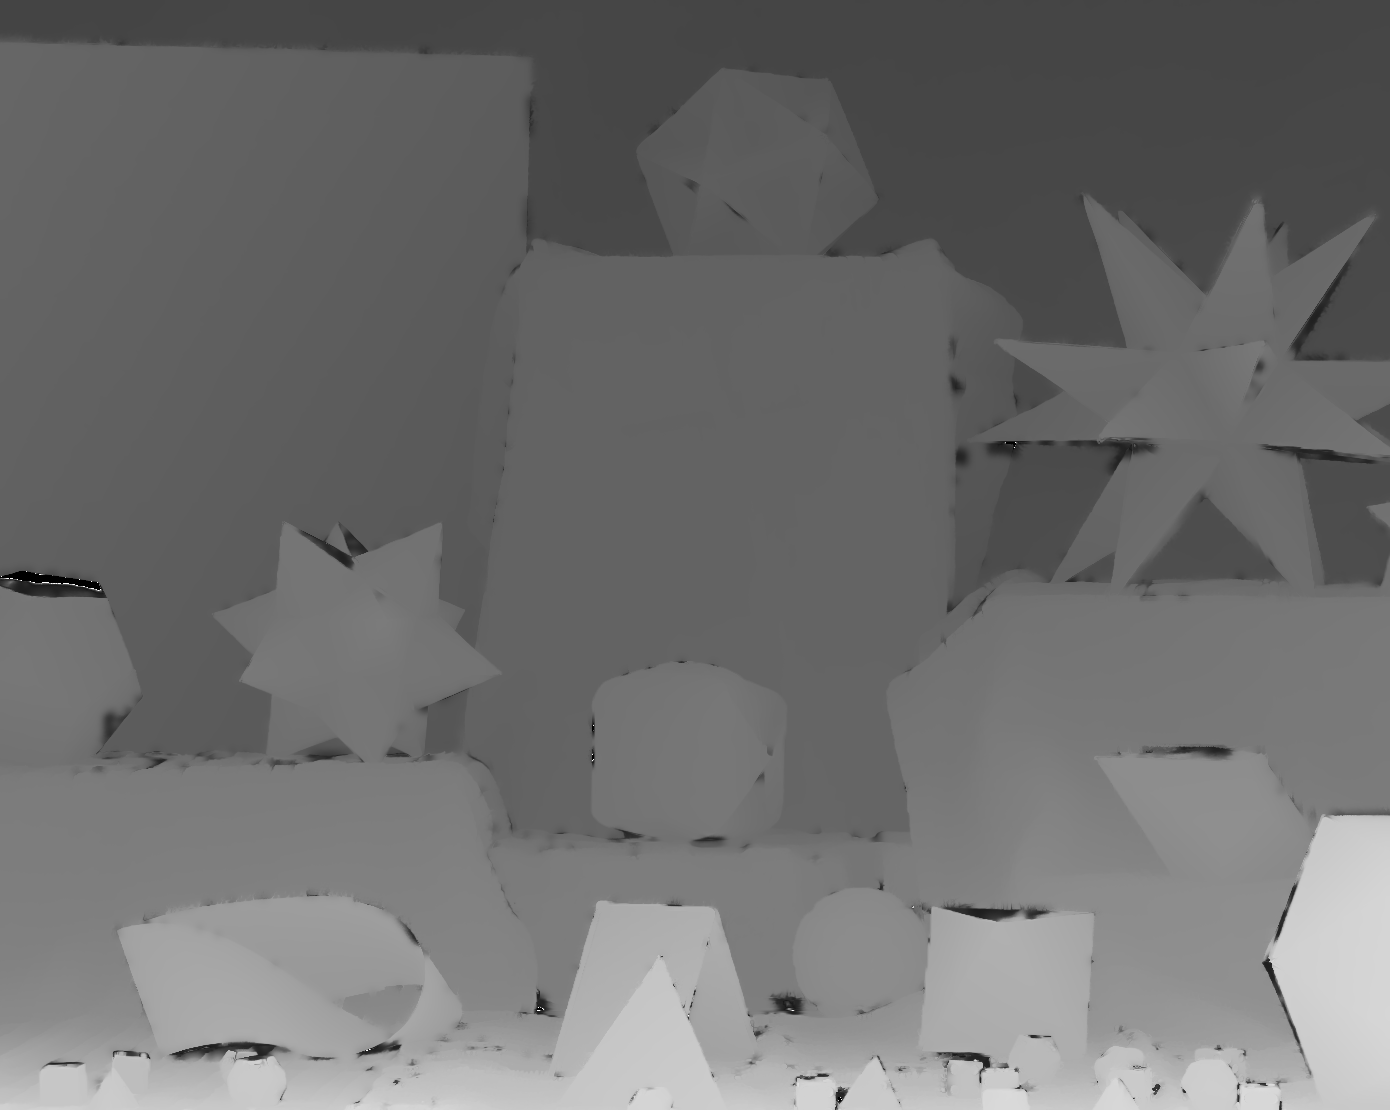
\includegraphics[width=5.5cm]{depth_interp/quan_nhf_moebius/yang.png}}
%  \vspace{1.5cm}
%   \centerline{(a)}\medskip
\end{minipage}
%
\hfill
\begin{minipage}[b]{0.48\linewidth}
  \centering
  \centerline{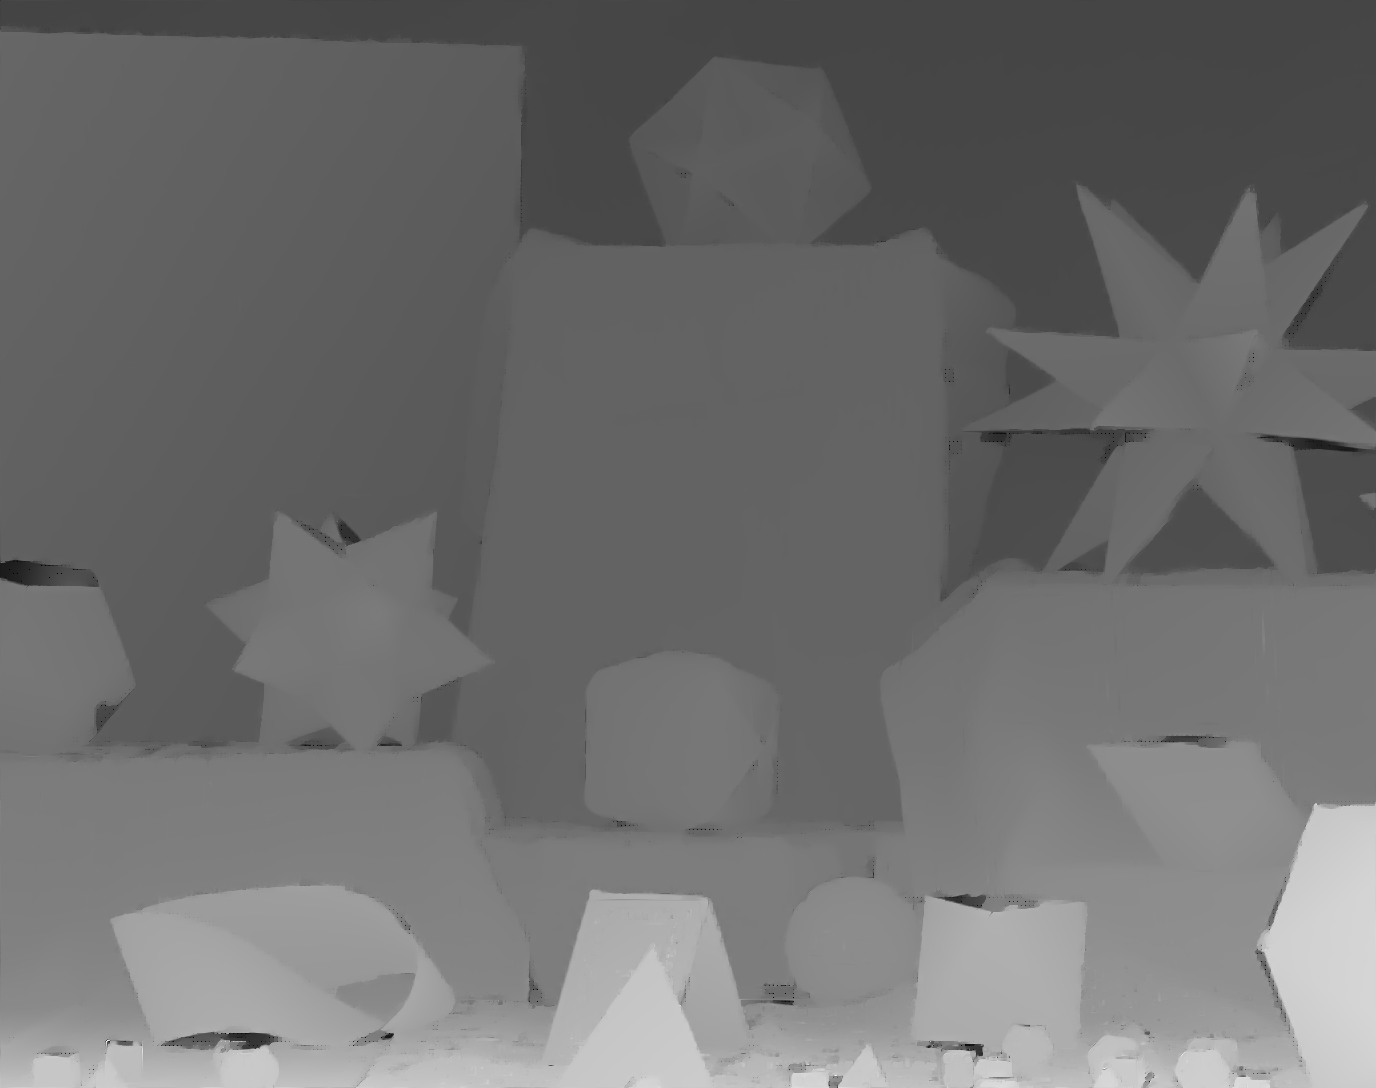
\includegraphics[width=5.5cm]{depth_interp/quan_nhf_moebius/tgv.png}}
%  \vspace{1.5cm}
%   \centerline{(a)}\medskip
\end{minipage}
%
\hfill
\begin{minipage}[b]{0.48\linewidth}
  \centering
  \centerline{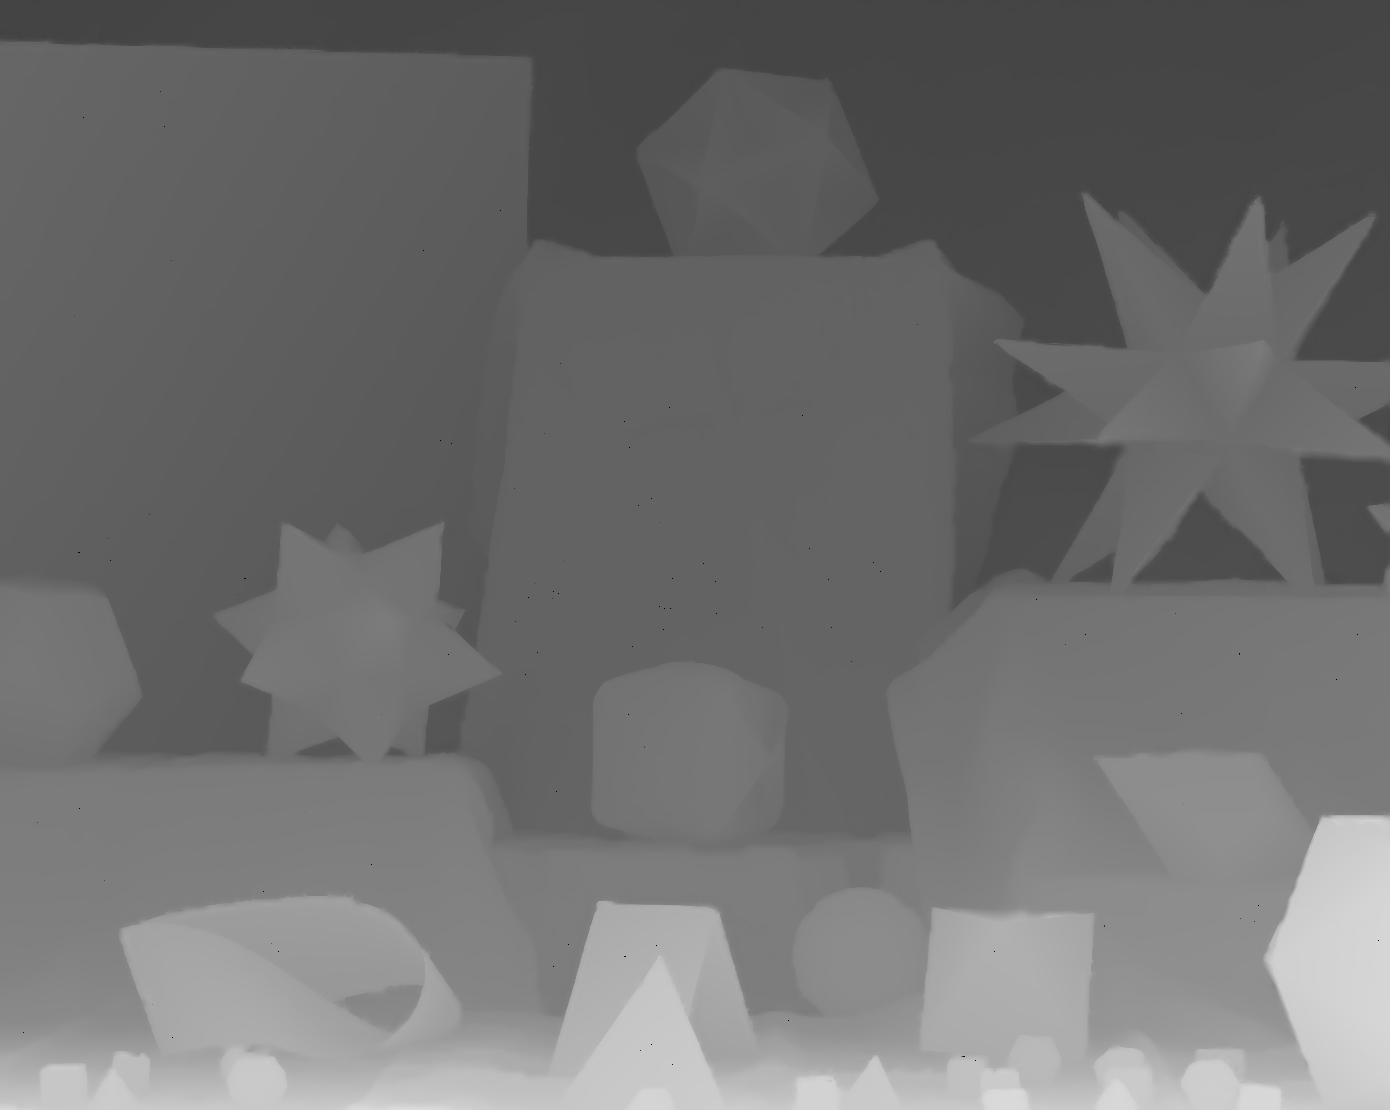
\includegraphics[width=5.5cm]{depth_interp/quan_nhf_moebius/our.png}}
%  \vspace{1.5cm}
%   \centerline{(b)}\medskip
\end{minipage}
\vfill
\caption{Visual comparison of different algorithm tested on Middlebury dataset~\cite{scharstein2003high} at $4\times$ upsampling rate. Column from left to right: RGB images, ground truth, and the results of: bilinear, bicubic, IBL~\cite{yang2014color}, TGV~\cite{ferstl2013image} and proposed; row from top to bottom: Art, Books, and Moebius.}
\label{fig:quan_rst}
\end{figure*}
\begin{landscape}
\begin{table*}[t]
\centering
\resizebox{1.4\textwidth}{!}{\begin{tabular}{|c|c|c|c|c|c|c|c|c|c|c|c|c|}
\hline & \multicolumn{12}{c|}{Images}   \\ \cline{2-13} 
& \multicolumn{4}{c|}{Art}          & \multicolumn{4}{c|}{Books}        & \multicolumn{4}{c|}{Moebius}      \\ \hline
\diagbox{\tiny{Methods}}{\tiny{Sample Rate}}   &     $2\times$     & $4\times$      & $8\times$      & $16\times$     & $2\times$       & $4\times$      & $8\times$      & $16\times$     & $2\times$      & $4\times$      & $8\times$     & $16\times$    \\ \hline
bicubic                                 & 0.8965 & 1.4298 & 2.4363 & 4.3456 & 0.7911 & 1.0842 & 1.7031 & 2.5419 & 0.6855 & 1.0287 & 1.5821 & 2.5527 \\ \hline
bilinear                                & 0.7642 & 1.2300 & 2.1495 & 3.9500 & 0.6620 & 0.8993 & 1.4183 & 2.1174 & 0.5685 & 0.8578 & 1.3347 & 2.1942 \\ \hline
% MRF~\cite{diebel2005application} & --     & --     & --     & --     & --     & --     & --     & --     & --     & --     & --     & --     \\ \hline
IBL~\cite{yang2007spatial}       & 0.5016 & 0.8934 & \bf{1.7028} & 4.2324 & 0.2790 & 0.7361 & 1.4056 & 2.4561 & 0.3987 & 0.7071 & 1.1289 & 2.5885 \\ \hline
TGV~\cite{ferstl2013image}       & 0.6457 & 0.8926 & 3.2633 & 7.6490  & 0.5980 & 0.7507 & 2.3091 & 6.324  & 0.4722 & 0.5627 & 2.0375 & 6.6210  \\ \hline
Proposed                                & \bf{0.4423} & \bf{0.8765} & 1.7616 & \bf{3.6033} & \bf{0.1986} & \bf{0.3594} & \bf{0.6655} & \bf{1.1888} & \bf{0.1864} & \bf{0.3426} & \bf{0.6478} & \bf{1.2393} \\ \hline
\end{tabular}}
\caption{Quantitative comparison of different algorithms tested on Middlebury dataset~\cite{scharstein2003high}. The results is evaluated as MAE (the smaller the better) for four different sample rates, as listed in the second row. All values are computed based on the disparity maps. The best result in each situation is in bold font.}
\label{table1}
\end{table*}
\end{landscape}
% \vspace*{-0.05in}
% \subsection{Quantitative Results}

Quantitative results comparing the proposed algorithm against prior work are obtained on the Middlebury stereo dataset 2005~\cite{scharstein2003high}. We first downsample the input depth map to obtain the low resolution version, and then run different algorithms on these images to obtain the upsampled versions. We use mean absolute error (MAE) as the metric to evaluate the performance of different algorithms. Table~\ref{table1} summarizes the results\footnote{Code for IBL implementation is provided by Chunhua Shen: https://bitbucket.org/chhshen/depth-enhancement.}. Fig.~\ref{fig:quan_rst} shows the corresponding visual results at the upsampling rate of 4. The results show that our algorithm is particularly suitable for depth map upsampling, and our algorithm provides a better result compared with the other algorithms. 

%The suitability for non hole filling depth map may be more appealing considering that the real condition usually comes with many missing points. 
% In this part we show the quantitative results of our results on the Middlebury stereo dataset 2005~\cite{scharstein2003high}. We first downsample the input depth map to obtain the low resolution version, and then run different algorithms on these images to obtain the upsampled versions. We use mean absolute error (MAE) as the metric to evaluate the performance of different algorithms. Table~\ref{table1} shows the results on the original Middlebury dataset without hole filling in advance, and Table~\ref{table2} shows the results of the hole filled version provided by~\cite{park2011high}. Fig.~\ref{fig:quan_rst} shows the corresponding visual results at upsampling rate of 4. The results show that our algorithm is robust on both situation and extremely suitable for non hole filling version, which may be more appealing considering that the real condition usually comes with many missing points. In both situation, our algorithm has a result reaching the level of state of art algorithms.

% \begin{table*}[ht]
% \centering
% \resizebox{0.98\textwidth}{!}{\begin{tabular}{|c|c|c|c|c|c|c|c|c|c|c|c|c|}
% \hline & \multicolumn{12}{c|}{Images}   \\ \cline{2-13} 
% & \multicolumn{4}{c|}{Art}          & \multicolumn{4}{c|}{Books}        & \multicolumn{4}{c|}{Moebius}      \\ \hline
% \diagbox{\tiny{Methods}}{\tiny{Sample Rate}}   &     $2\times$     & $4\times$      & $8\times$      & $16\times$     & $2\times$       & $4\times$      & $8\times$      & $16\times$     & $2\times$      & $4\times$      & $8\times$     & $16\times$    \\ \hline
% bicubic           & 0.6218 & 1.0752 & 1.9778 & 3.7035 & 0.2360  & 0.3863 & 0.6732 & 1.2362 & 0.2423 & 0.3707 & 0.6645 & 1.2030 \\ \hline
% bilinear          & 0.5670 & 0.9774 & 1.8257 & 3.4853 & 0.2138  & 0.3482 & 0.6087 & 1.1290 & 0.2423 & 0.4007 & 0.7112 & 1.2715 \\ \hline
% MRF~\cite{diebel2005application}               & 0.6250 & 1.0052 & 1.9741 & 3.9370 & 0.2167  & 0.3332 & 0.6162 & 1.2107 & 0.2502 & 0.3679 & 0.6731 & 1.2884 \\ \hline
% IBL~\cite{yang2007spatial}              & 0.5709 & 0.7002 & 1.5046 & 3.6903 & 0.30130 & 0.4514 & 0.6373 & 1.4532 & 0.3868 & 0.4760 & 0.6893 & 1.1366 \\ \hline
% TGV~\cite{ferstl2013image}               & 0.5121 & 0.7842 & 2.4615 & 7.2681 & 0.2085  & 0.3470 & 1.1474 & 3.8096 & 0.1949 & 0.3221 & 1.1860 & 3.6391 \\ \hline
% Proposed              & 0.4652 & 0.9098 & 1.8183 & 3.6754 & 0.2142  & 0.3702 & 0.6688 & 1.2404 & 0.1958 & 0.3575 & 0.6674 & 1.2570 \\ \hline
% \end{tabular}}
% \caption{Quantitative comparison of different algorithms tested on Middlebury dataset with hole filled provided by~\cite{park2011high}. The results is evaluated as MAD (the smaller the better) for four different sample rates, as listed in the second row. All values are computed based on the disparity maps. The images of MRF~\cite{diebel2005application} and IBL~\cite{yang2007spatial} are provided by~\cite{park2011high}.}
% MAE (the smaller the better) of three images of the hole filled version in~\cite{park2011high}. The second row is the upsampling rate. All values are computed based on the disparity maps. The metric of MRF~\cite{diebel2005application} and IBL~\cite{yang2014color} are provided by~\cite{park2011high}}
% \label{table2}
% \end{table*}
% \begin{figure*}[ht]
% \begin{minipage}[b]{0.13\linewidth}
%   \centering
%   \centerline{\includegraphics[width=2.4cm]{quan_hf/Art.png}}
% %  \vspace{1.5cm}
% %   \centerline{(a)}\medskip
% \end{minipage}
% %
% \hfill
% \begin{minipage}[b]{0.13\linewidth}
%   \centering
%   \centerline{\includegraphics[width=2.4cm]{quan_nhf/gt.png}}
% %  \vspace{1.5cm}
% %   \centerline{(a)}\medskip
% \end{minipage}
% \hfill
% \begin{minipage}[b]{0.13\linewidth}
%   \centering
%   \centerline{\includegraphics[width=2.4cm]{quan_nhf/bl.png}}
% %  \vspace{1.5cm}
% %   \centerline{(a)}\medskip
% \end{minipage}
% %
% \hfill
% \begin{minipage}[b]{0.13\linewidth}
%   \centering
%   \centerline{\includegraphics[width=2.4cm]{quan_nhf/bc.png}}
% %  \vspace{1.5cm}
% %   \centerline{(b)}\medskip
% \end{minipage}
% \hfill
% \begin{minipage}[b]{0.13\linewidth}
%   \centering
%   \centerline{\includegraphics[width=2.4cm]{quan_nhf/yang.png}}
% %  \vspace{1.5cm}
% %   \centerline{(a)}\medskip
% \end{minipage}
% %
% \hfill
% \begin{minipage}[b]{0.13\linewidth}
%   \centering
%   \centerline{\includegraphics[width=2.4cm]{quan_nhf/tgv.png}}
% %  \vspace{1.5cm}
% %   \centerline{(a)}\medskip
% \end{minipage}
% %
% \hfill
% \begin{minipage}[b]{0.13\linewidth}
%   \centering
%   \centerline{\includegraphics[width=2.4cm]{quan_nhf/our.png}}
% %  \vspace{1.5cm}
% %   \centerline{(b)}\medskip
% \end{minipage}
% \vfill
% \begin{minipage}[b]{0.13\linewidth}
%   \centering
%   \centerline{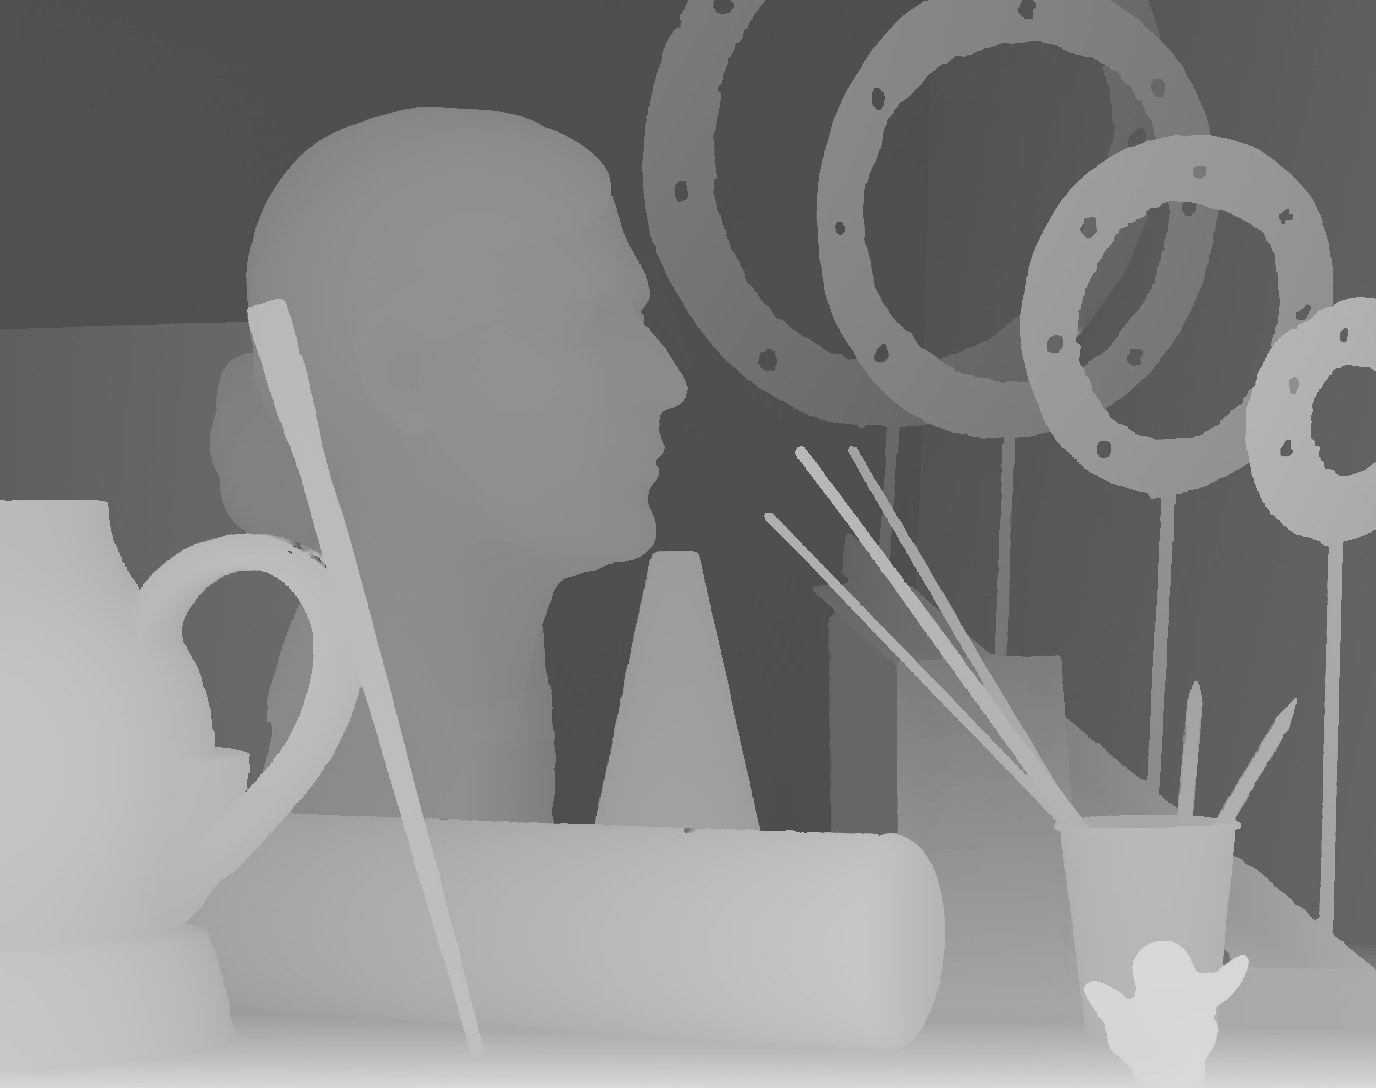
\includegraphics[width=2.4cm]{quan_hf/gt.png}}
% %  \vspace{1.5cm}
% %   \centerline{(c)}\medskip
% \end{minipage}
% \hfill
% \begin{minipage}[b]{0.13\linewidth}
%   \centering
%   \centerline{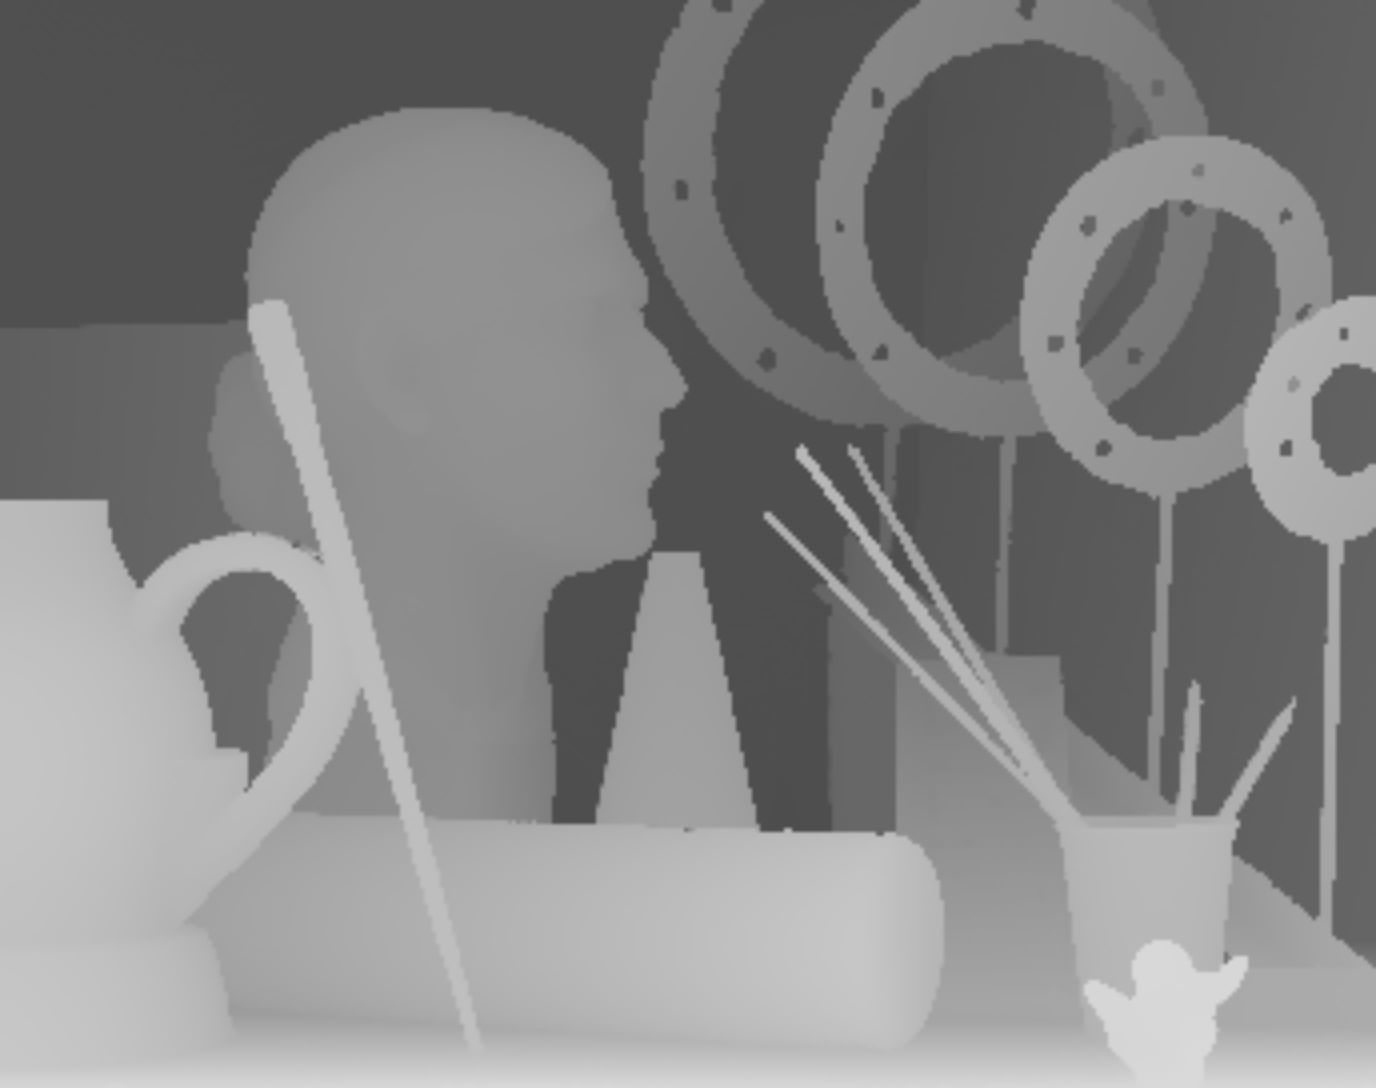
\includegraphics[width=2.4cm]{quan_hf/bl.png}}
% %  \vspace{1.5cm}
% %   \centerline{(a)}\medskip
% \end{minipage}
% %
% \hfill
% \begin{minipage}[b]{0.13\linewidth}
%   \centering
%   \centerline{\includegraphics[width=2.4cm]{quan_hf/bc.png}}
% %  \vspace{1.5cm}
% %   \centerline{(b)}\medskip
% \end{minipage}
% \hfill
% \begin{minipage}[b]{0.13\linewidth}
%   \centering
%   \centerline{\includegraphics[width=2.4cm]{quan_hf/mrf.png}}
% %  \vspace{1.5cm}
% %   \centerline{(c)}\medskip
% \end{minipage}
% \hfill
% \begin{minipage}[b]{0.13\linewidth}
%   \centering
%   \centerline{\includegraphics[width=2.4cm]{quan_hf/yang.png}}
% %  \vspace{1.5cm}
% %   \centerline{(a)}\medskip
% \end{minipage}
% %
% \hfill
% \begin{minipage}[b]{0.13\linewidth}
%   \centering
%   \centerline{\includegraphics[width=2.4cm]{quan_hf/tgv.png}}
% %  \vspace{1.5cm}
% %   \centerline{(a)}\medskip
% \end{minipage}
% %
% \hfill
% \begin{minipage}[b]{0.13\linewidth}
%   \centering
%   \centerline{\includegraphics[width=2.4cm]{quan_hf/our.png}}
% %  \vspace{1.5cm}
% %   \centerline{(b)}\medskip
% \end{minipage}
% \vfill
% \caption{Visual comparison of different algorithm tested on Middlebury dataset~\cite{scharstein2003high} at $4\times$ upsampling rate. Top from left to right: RGB image of Art, non hole filled ground truth, and the results of: bilinear, bicubic, IBL~\cite{yang2014color}, TGV~\cite{ferstl2013image} and ours; bottom from left tot right: hole filled ground truth~\cite{park2011high}, and the results of: bilinear, bicubic, MRF~\cite{diebel2005application}, IBL~\cite{yang2014color}, TGV~\cite{ferstl2013image} and ours.}
% \label{fig:quan_rst}
% \end{figure*}

\subsection{Discussion}
\label{sec:2.discussion}
%The proposed algorithm is based on the assumption that for a small patch, the depth values are linear in the spatial coordinates and the edges on depth map are controlled by the corresponding RGB image. 
Table~\ref{table1} illustrates that the depth map upsampling obtained with the proposed algorithm is accurate and achieves the state of the art results on the common benchmarking dataset, providing a better performance compared with other algorithms. The proposed algorithm, however, still suffers from two limitations. First, there are a few outlier points where the method yields a large error. Second, the edges are not sharply defined, especially under high upsampling rate, which is typical in most depth upsampling algorithms. The computational requirements are an additional challenge: to process a $1088\times 1296$ pixel image, our algorithm takes about 40min. While the time requirement is analogous for several other upsampling algorithms, a speed-up is desirable for many applications. 

We also want to mention more about the relation of the proposed algorithm with Levin's~\cite{levin2008closed} matting method and He's~\cite{he2010fast} fast computing algorithm. Levin's method is to formulate a linear combination of neighbour pixels value for estimating matting map, or alpha channel; He's method is based on Levin's formulation and proposed the acceleration also using conjugate gradient. In our problem, we utilize the linear relation of spacial instead direct pixel values; and, we formulate a local filtered conjugate gradient formulation using conjugate gradient, instead of an adjacent matrix. The similarity and difference of the proposed algorithm with Levin's method is listed in~\ref{table:relation_matting}.  

\begin{table}[htb]
\centering
\resizebox{0.98\textwidth}{!}{
\begin{tabular}[c]{l|l|l}
 & Levin's matting method    & Proposed method
 \\ \hline
similarity & \multicolumn{2}{l}{\begin{tabular}{l}\tabitem linear model\\
\tabitem build Laplacian matrix to solve the optimization\end{tabular}}           \\ \hline
difference & linear in color intensity & \begin{tabular}{l} \tabitem linear in relative spatial location\\ \tabitem weight based on color information\end{tabular}
\end{tabular}}
\caption{Similarity and difference of the proposed algorithm with Levin's method~\cite{levin2008closed.}}
\label{table:relation_matting}
\end{table}

%the challenging because it is both application and content dependent.

% Our algorithm is based on the assumption that in a small patch, the depth values are linear and the edges on depth map are controlled by the corresponding RGB image. From Table~\ref{table1} and Table~\ref{table2} we find that the depth map upsampling is accurate at low upsampling rate and achieves the state of the art results on the common benchmarking dataset. Meanwhile, through the comparison of the two tables, our algorithm proves a better performance on non hole filling version which may be more accustomed to actual usage. However, this algorithm still suffers from two problems. First, there are some bad point with very low disparity value after the interpolation. Second, the edge, especially under high upsampling rate, is not satisfying, which is typical in most depth upsampling algorithms. Meanwhile, to process an image with resolution $1088\times 1296$, our algorithm takes about 40min, which is time consuming as many other depth upsampling algorithms. In our future work, we aim at alleviating these problems by implementing some post processing using segmentation techniques, and use techniques such as a coarse to fine structure~\cite{Chao:Colorization:pspie9020} to accelerate the computing.

\section{Conclusion}
\label{sec:2.conclusion}
%In this paper we propose a novel algorithm for both low resolution depth map upsampling and high resolution depth map hole filling. 

The algorithm proposed in this paper provides an effective method for depth map upsampling and hole filling. Quantitative results on test data indicates that the method offers an improvement over current state of the art methods and visual assessment shows that the depth map estimated by the proposed technique is consistent with the color images.

% Compared to several the state of the art, our proposed algorithm offers improved accuracy

%Our algorithm assumes a linear relation in patches of the depth map, and optimizes an objective constructed on the weighted linear fitting. We showed the qualitative and quantitative experiments of our algorithm and the comparison with other algorithms. The result shows that our algorithm reach the level of state of art algorithms and extremely suitable for depth map upsampling with many missing points.

%%% Local Variables: 
%%% mode: latex
%%% TeX-master: "dissertation"
%%% End: 
\setcounter{section}{0}
\let\oldthesection\thesection
\renewcommand{\thesection}{\thechapter.\Alph{section}}
\section{Appendix to Chapter~\ref{sec2.3.2}}
\label{ap1}
For ~\eqref{eq:2.6},
\begin{equation}
\begin{split}
P_{j} &=  {\argmin}_{P_{j}}{((W_{j}(D_{H,N_{j}}-GP_{j}^T))^2)}\\
&= (G^{T}W_{0,j}^{T}G)^{-1}G^{T}W_{0,j}^{T}D_{H,N_{j}},
\end{split}
\end{equation}
so,
\begin{equation}
\begin{split}
d((W_{j}(D_{H,N_{j}}-GP_{j}^T))^2)/dP_{j} &= 0\\
&= W_{j}(D_{H,N_{j}}-GP_{j}^T))G^T,
\end{split}
\end{equation}
solve the linear equation gives,
\begin{equation}
P_{j} = (G^{T}W_{0,j}^{T}G)^{-1}G^{T}W_{0,j}^{T}D_{H,N_{j}}.
\end{equation}

For ~\eqref{eq:2.7},
\begin{equation}
\begin{split}
Q &= \sum_{j=1}^{N}{(W_{j}(D_{H,N_{j}}-G{(G^{T}W_{0,j}^{T}G)^{-1}G^{T}W_{0,j}^{T}D_{H,N_{j}}}^T))^2+{\lambda}F_{j}}\\
&= \sum_{j=1}^{N}{((W_{j}D_{H,N_{j}})(E-G{(G^{T}W_{0,j}^{T}G)^{-1}G^{T}W_{0,j}^{T}}^T))^2+{\lambda}F_{j}}\\
&= \sum_{j=1}^{N}{D_{H,N_{j}}^{T}(\overline{G_{j}}^{T}W_{0,j}\overline{G_{j}})D_{H,N_{j}}}+{\lambda}F_{j}\\
&= \sum_{j=1}^{N}{D_{H,N_{j}}^{T}(\overline{G_{j}}^{T}W_{0,j}\overline{G_{j}})D_{H,N_{j}}}+\sum_{j=1}^{M}{\lambda(D_{L,j}-D_{H,j})^2},
\end{split}
\label{eq:2.7}
\end{equation}


\renewcommand{\thesection}{\thechapter.\Alph{section}}
\section{Appendix to Chapter~\ref{sec2.3.3}}
\label{ap2}
For~\eqref{eq:2.cgs_final},
\begin{equation}
\begin{split}
(Lp)_{i} &= \sum{\delta_{ij}w_{ki}P_{i}}-G_{i}\sum_{k\in N_{i}}{a_{k}w_{ki}}+\sum_{k\in N_{i}}{b_{k}w_{ki}}\\
&= \sum{\delta_{ij}w_{ki}P_{i}}-G_{i}\sum_{k\in N_{i}}{a_{k}w_{ki}k_{0}a_{k}w_{ki}}\\
&= \sum{\delta_{ij}w_{ki}P_{i}}-G_{i}\sum_{k\in N_{i}}{(C_{k}(\sum_{j\in N_{k}}{w_{kj}}G_{j}P_{j}-k\overline{p_{k}}))w_{ki}k_{0}a_{k}w_{ki}}\\
& = \sum_{j}{(\sum_{k|i,j\in N_{k}}{(\delta_{ij}w_{ki}-w_{ki}w_{kj}(G_{i}-k_{0})C_{k}(G_{j}-k_{0}))})p_j},
\end{split}
\end{equation}
which demonstrates the consistency of two different expression.
% Go back to the old section numbering for future chapters
\let\thesection\oldthesection